\documentclass[11pt,a4paper]{article}
\usepackage[italian]{babel}
\usepackage[utf8]{inputenc}
\usepackage[T1]{fontenc}
\usepackage{calligra}
\usepackage{makeidx}
\usepackage{hyperref}
\usepackage{amsmath}
\usepackage{amsfonts}
\usepackage{amssymb}
\usepackage{makeidx}
\usepackage{graphicx}
\usepackage{wrapfig}
\usepackage{amsmath}
\usepackage{enumerate}
\usepackage{subfigure}
\usepackage{fancyhdr}
\usepackage{amsthm}
\usepackage{amsfonts}
\usepackage[a4paper, inner=1.5cm, outer=3cm, top=3cm, 
bottom=3cm, bindingoffset=1cm]{geometry} 

\begin{document}
\title{Soluzione numerica delle equazioni di Kohn-Sham} 
\author{Simone Orioli} 
\date{Anno Accademico 2013/2014} 
\maketitle
\tableofcontents
\newpage

\section{Introduzione teorica}
\subsection{Equazioni di Kohn-Sham}
Data l'Hamiltoniana di un sistema a molti corpi
\begin{equation}
\mathcal{\hat{H}} = -\frac{\hbar^2}{2m}\sum_{i=1}^N \nabla_i^2 + \sum_{i=1}^N v_{ext}(\textbf{r}_i) + \frac{1}{2}\sum_{i\not=j}^N v(r_{ij}) = \hat{T} + V_{ext} + V_{int}
\end{equation} 
la teoria del \emph{funzionale densità} prevede, stando al teorema di Kohn-Hoenberg, la possibilità di esprimere l'energia di ground-state di tale sistema come
\begin{equation}
E_{GS} = \int d^3 r V_{ext}(\textbf{r})\rho_{GS}(\textbf{r}) + F[\rho_{GS}]
\end{equation}
dove $F[\rho]$ è il \emph{funzionale di Levy}, definito come
\begin{equation}
F[\rho] := \min_{\psi \to \rho} \langle \psi | \hat{T} + V_{int} | \psi \rangle
\end{equation}
dove il minimo è da intendersi come il minimo sulle funzioni d'onda che generano una determinata densità $\rho$. In particolare, per densità $\rho$ di un sistema a $N$ corpi intendiamo la solita densità a $N$-corpi normalizzata al numero di particelle:
\[
\rho(\textbf{r}) = N \int d^3r_2\ldots d^3r_N |\psi(\textbf{r}_1,\textbf{r}_2,\ldots ,\textbf{r}_N)|^2
\]
L'efficacia del teorema di Kohn-Hoenberg risiede nel fatto che il funzionale densità ci permette di dimenticare i dettagli dell'Hamiltoniana, ma al prezzo di una scrittura approssimata di $F[\rho]$. Infatti, la conoscenza della forma esatta di tale funzionale è equivalente alla conoscenza della soluzione del problema: in questo senso una scrittura analitica di $F[\rho]$ è impredicibile.
\\
Per un sistema fermionico, Kohn e Sham hanno proposto la scrittura del funzionale energia, genericamente inteso come
\[
E[\rho] = \int d^3 r V_{ext}(\textbf{r})\rho(\textbf{r}) + F[\rho] \geq E_{GS}
\]
nella seguente forma
\begin{equation}
E[\rho] = T_0(\rho) + \int d^3r \rho(\textbf{r}) \left( V_{ext}(\textbf{r})+\frac{1}{2}U(\textbf{r}) \right) + E_{xc}(\rho)
\end{equation}
dove con $T_0(\rho)$ intendiamo l'energia cinetica di un sistema di particelle non interagenti con densità $\rho$, con $U(\textbf{r})$ il cosiddetto \emph{potenziale di Hartree}, ottenuto come
\[
U(\textbf{r}) = \int d^3r' \rho(\textbf{r}')v(|\textbf{r}-\textbf{r}'|)
\]
e con $E_{xc}$ l'\emph{energia di scambio-correlazione}. A partire da questo funzionale energia possiamo ricavare le \emph{equazioni di Kohn-Sham} tramite un approccio variazionale, fissando il numero di particelle nel sistema attraverso un moltiplicatore di Lagrange $\varepsilon_i$ e calcolando
\begin{equation}
\frac{\delta}{\delta \varphi_i^*} ( E[\rho] - \varepsilon_i N) = 0
\end{equation}
intendendo con $\varphi_i$ le funzioni di singola particella del ground state del nostro sistema fermionico, la cui funzione d'onda è espressa tramite il determinante di Slater
\[
\Psi(\textbf{r}_1,\ldots \textbf{r}_N) = \det S(\varphi_1, \ldots , \varphi_N)
\]
Il fatto che i moltiplicatori di Lagrange siano diversi per ogni funzione d'onda di singola particella è dovuto al fatto che i fermioni, al contrario dei bosoni, non occupano tutti un singolo stato, ma piuttosto si dispongono su stati a diverse energie: teniamo conto di questo effetto attribuendo a ciascuna $\varphi_i$ un diverso moltiplicatore $\varepsilon_i$. Si ottiengono così le \emph{equazioni di Kohn-Sham}:
\begin{equation}
-\frac{\hbar^2}{2m}\nabla^2\varphi_i(\textbf{r}) + V_{ext}(\textbf{r})\varphi_i(\textbf{r}) + \left( \int d^3r' \rho(\textbf{r})v(|\textbf{r}-\textbf{r}'|) \right)\varphi_i(\textbf{r}) + \frac{\partial E_{xc}(\rho(\textbf{r}))}{\partial \rho}\varphi_i(\textbf{r}) = \varepsilon_i \varphi_i(\textbf{r})
\end{equation} 
ovvero un set di equazioni di singola particella da risolvere per ogni fermione che compone il sistema. Da queste equazioni si può osservare che
\[
\sum_{i=1}^N \varepsilon_i = E[\rho] - E_{xc}(\rho) + \left\langle \frac{\partial E_{xc}}{\partial \rho} \right\rangle + \frac{1}{2}\langle U \rangle
\]
ovvero che, una volta ricavata numericamente la corretta densità del sistema è possibile calcolare l'energia del ground state come
\begin{equation}\label{7}
E[\rho] = \sum_{i=1}^N \varepsilon_i + E_{xc}(\rho) - \left\langle \frac{\partial E_{xc}}{\partial \rho} \right\rangle - \frac{1}{2}\langle U \rangle
\end{equation}
\subsection{Local density approximation (LDA)}
Per un sistema la cui densità varia lentamente con la distanza, l'energia di scambio-correlazione può essere espressa come
\begin{equation}
E_{xc}(\rho) = \int d^3r \rho(\textbf{r}) \varepsilon_{xc}(\rho(\textbf{r}))
\end{equation}
dove $\varepsilon_{xc}(\rho(\textbf{r}))$ è l'energia di scambio-correlazione per particella di un sistema uniforme con densità $\rho$, ovvero $\varepsilon_{xc}(\rho) = E_{xc}(\rho)/N$. Tale approssimazione è nota come \emph{approssimazione di densità locale} o \emph{LDA (local density approximation)}. Inoltre è possibile separare i due contributi di scambio e correlazione:
\begin{equation}
\varepsilon_{xc}(\rho(\textbf{r})) = \varepsilon_{x}(\rho(\textbf{r})) + \varepsilon_c(\rho(\textbf{r})) 
\end{equation}
che possono essere calcolati il primo esplicitamente e il secondo attraverso l'utilizzo di metodi Monte Carlo. A riguardo del termine di scambio, se supponiamo che i fermioni nel sistema (tridimensionale) interagiscano tramite potenziale coulombiano
\[
v(r_{ij}) = \frac{e^2}{|\textbf{r}_i-\textbf{r}_j|}
\]
si ottiene
\begin{equation}
\varepsilon_{x}^{3D}(\rho(\textbf{r})) = -\frac{3}{4}\left( \frac{3}{\pi} \right)^{1/3}\rho^{1/3}(\textbf{r})
\end{equation}
Per quanto riguarda l'energia di correlazione, se definiamo il \emph{raggio di Wiegner-Seitz} come il raggio della sfera il cui volume è pari al volume tipico occupato da una particella, ossia 
\[
V_t = \frac{4}{3}\pi r_s^3 \Longrightarrow V_t = \frac{1}{\rho(\textbf{r})} \Longrightarrow r_s = \sqrt[3]{\frac{3}{4\pi \rho(\textbf{r})}}
\]
otteniamo
\begin{equation}
\varepsilon_c(\rho(\textbf{r})) = -\frac{0.44}{7.8 +r_s}
\end{equation}
In questo approccio, l'equazione \eqref{7} può essere riscritta in una maniera più semplice. Otteniamo infatti
\[
\begin{split}
E[\rho] &= \sum_{i=1}^N \varepsilon_i - \frac{1}{2}\int d^3r U(\textbf{r}) \rho(\textbf{r}) - \int d^3r \frac{\partial E_{xc}(\rho)}{\partial \rho}\rho(\textbf{r}) + \int d^3r \varepsilon_{xc}(\rho)\rho(\textbf{r}) \\
&= \sum_{i=1}^N \varepsilon_i - \frac{1}{2}\int d^3r U(\textbf{r}) \rho(\textbf{r}) - \int d^3r \left( \frac{\partial \varepsilon_{xc}(\rho)}{\partial\rho}\rho(\textbf{r}) - \varepsilon_{xc}(\rho) \right)\rho(\textbf{r}) + \int d^3r \varepsilon_{xc}(\rho)\rho(\textbf{r}) \\
&= \sum_{i=1}^N \varepsilon_i - \frac{1}{2}\int d^3r U(\textbf{r}) \rho(\textbf{r}) - \int d^3r \frac{\partial \varepsilon_{xc}(\rho)}{\partial\rho}\rho^2(\textbf{r})
\end{split}
\]
dove, per calcolo diretto si ha
\[
\frac{\partial \varepsilon_{xc}(\rho)}{\partial\rho}\rho^2(\textbf{r}) = -\frac{1}{4}\left( \frac{3}{\pi}\right)^{1/3}\rho^{4/3}(\textbf{r}) - \frac{1}{3}\frac{0.44}{(7.8+r_s)^2}\left( \frac{3}{4\pi} \right)^{1/3}\rho^{2/3}(\textbf{r})
\]
\subsection{Potenziali esterno e di Hartree}
Per quanto riguarda il potenziale di interazione (Hartree) è possibile svolgere il conto esplicito, sempre supponendo che l'interazione tra i fermioni sia coulombiana e con l'ulteriore ipotesi che la densità dipenda solo dal modulo del raggio $r=|\textbf{r}|$, ottenendo
\begin{equation}
U(\textbf{r}) = \int d^3r' \frac{\rho(\textbf{r}')}{|\textbf{r}-\textbf{r}'|} = \frac{4\pi}{r} \int _0^r dr' \rho(r') r'^2 + 4\pi \int _r^{+\infty}dr' \rho(r') r'
\end{equation}
Il potenziale esterno, invece, può essere pensato come generato da una sfera carica di raggio $R_c$ e densità di carica uniforme
\[
\rho_+ = \frac{3Ne}{4\pi R_c^3}
\]
In questo modo, utilizzando il teorema di Gauss si può calcolare il potenziale generato da tale sfera carica, dato da
\begin{equation}
V_{ext}(r) = 2\pi \rho_+ \begin{cases}
\frac{1}{3}r^2 - R_c^3 \quad &\text{se} \quad r < R_c \\
-\frac{2}{3}\frac{R_c^3}{r} \quad &\text{se} \quad r\geq R_c
\end{cases}
\end{equation}
Per garantire la neutralità del sistema scegliamo $R_c = r_s \sqrt[3]{N}$. 

\section{Metodi numerici}
\subsection{Algoritmo di diagonalizzazione}
Consideriamo la seguente equazione di Schr\"{o}dinger unidimensionale:
\begin{equation}\label{14}
-\frac{\hbar^2}{2m}\frac{d^2\psi(x)}{dx^2} + V(x)\psi(x)=E\psi(x)
\end{equation}
dove $V(x)$ è un generico potenziale che può tenere conto, in generale, anche di contributi efficaci. Per ottenere un algoritmo numerico di risoluzione per questa equazione, possiamo cominciare definendo una griglia numerica $[x_0,x_N]$ di passo $\Delta x$ e le seguenti notazioni:
\begin{align*}
\psi(x_{i+1}) \equiv \psi(x_i + \Delta x)  \\
\psi(x_{i-1}) \equiv \psi(x_i - \Delta x)
\end{align*}
Possiamo discretizzare la derivata seconda sulla griglia sviluppando in serie di Taylor le due funzioni $\psi(x+\Delta x)$ e $\psi(x-\Delta x)$:
\begin{align*}
\psi(x_{i+1}) = \psi(x_i) + \frac{d\psi(x_i)}{dx}\Delta x + \frac{d^2 \psi(x_i)}{dx^2}(\Delta x)^2 + o[(\Delta x)^3] \\
\psi(x_{i-1}) = \psi(x_i) - \frac{d\psi(x_i)}{dx}\Delta x + \frac{d^2 \psi(x_i)}{dx^2}(\Delta x)^2 + o[(\Delta x)^3]
\end{align*}
Sommando membro a membro si ottiene un'espressione discretizzata della derivata con precisione dell'ordine di $o(\Delta x)$:
\begin{equation}
\frac{d^2 \psi(x_i)}{dx^2} = \frac{\psi(x_{i+1}) - 2\psi(x_i) + \psi(x_{i-1})}{(\Delta x)^2} + o(\Delta x)
\end{equation}
L'equazione \eqref{14} in forma discretizzata è dunque data da:
\begin{equation}
-\frac{\hbar^2}{2m} \left( \frac{\psi(x_{i+1}) - 2\psi(x_i) + \psi(x_{i-1})}{(\Delta x)^2} \right) + V(x_i)\psi(x_i) = E\psi(x_i)
\end{equation}
Questa espressione suggerisce la seguente riscrittura dell'equazione in forma matriciale:
\[
\begin{split}
\left( \begin{array}{cccccc}
V(x_1) + \frac{\hbar^2}{m(\Delta x)^2} & -\frac{\hbar^2}{2m(\Delta x)^2} & 0 & \ldots & \ldots & \ldots  \\
-\frac{\hbar^2}{2m(\Delta x)^2} & V(x_2) + \frac{\hbar^2}{m(\Delta x)^2} & -\frac{\hbar^2}{2m(\Delta x)^2} & 0 & \ldots & \ldots \\
0 & -\frac{\hbar^2}{2m(\Delta x)^2} & V(x_2) + \frac{\hbar^2}{m(\Delta x)^2} & -\frac{\hbar^2}{2m(\Delta x)^2} & 0 & \ldots \\
\vdots & \ddots & \ddots & \ddots & \vdots & \vdots \\
\end{array}\right) 
\left( \begin{array}{c}
\psi(x_1) \\ \vdots \\ \vdots \\ \psi(x_N)
\end{array} \right)  
\end{split}
\]
\[
\\ 
 = E\left( \begin{array}{c}
\psi(x_1) \\ \vdots \\ \vdots \\ \psi(x_N)
\end{array} \right)
\]
Conseguentemente, il problema della risoluzione dell'equazione di Schr\"{o}dinger si riduce al problema della diagonalizzazione di una matrice. Esistono delle routine ottimizzate per la risoluzione di problemi agli autovalori, ed in questo caso, per la diagonalizzazione della matrice appena discussa, è stata utilizzata la funzione $eig\_sim()$ fornita dalla libreria \emph{Armadillo} per C++. 
%\\ \ \\
%La procedura di diagonalizzazione presenta però un problema fondamentale: il tempo di calcolo scala in maniera non lineare con la dimensione della matrice. Evidentemente l'efficacia del metodo appena sviluppato per la risoluzione dell'equazione di Schr\"{o}dinger è tanto più preciso quanto maggiore è la dimensione della matrice (in quanto, fissato il raggio massimo entro il quale si sceglie di studiare il sistema, maggiore è la dimensione della matrice minore sarà il valore di $\Delta x$), e conseguentemente la precisione dei nostri risultati risulterà fortemente vincolata dai tempi computazionali che siamo disposti ad accettare. In più, le equazioni di Kohn-Sham richiederanno, per essere risolte, una procedura iterativa basata sul metodo autoconsistente, e di conseguenza è fondamentale che la singola iterazione non richieda un ammontare di tempo esagerato. Per studiare il comportamento dell'algoritmo fornito dalla libreria GSL è stata risolta l'equazione di Schr\"{o}dinger per l'oscillatore armonico tridimensionale,
%\[
%\left(-\frac{d^2}{dr^2} + \frac{1}{2}r^2 \right)\psi(r) = E\psi(r)
%\] 
%di cui si conosce la soluzione analitica: in questo modo è stato possibile valutare in che modo il risultato della diagonalizzazione risulti vincolato alla dimensione della matrice. Per la risoluzione è stato scelta una griglia numerica $[R_0,R_{max}] = [0,25]$ (identica a quella che verrà utilizzata in seguito per le equazioni di Kohn-Sham) ed un $\Delta x$ variabile dipendentemente dalla dimensione desiderata per la matrice. In figura vengono mostrati i risultati ottenuti. 
%\begin{figure}[!h]
%\centering
%\subfigure[Andamento del tempo di computazione in funzione della dimensione della matrice (in scala logaritmica)]
%{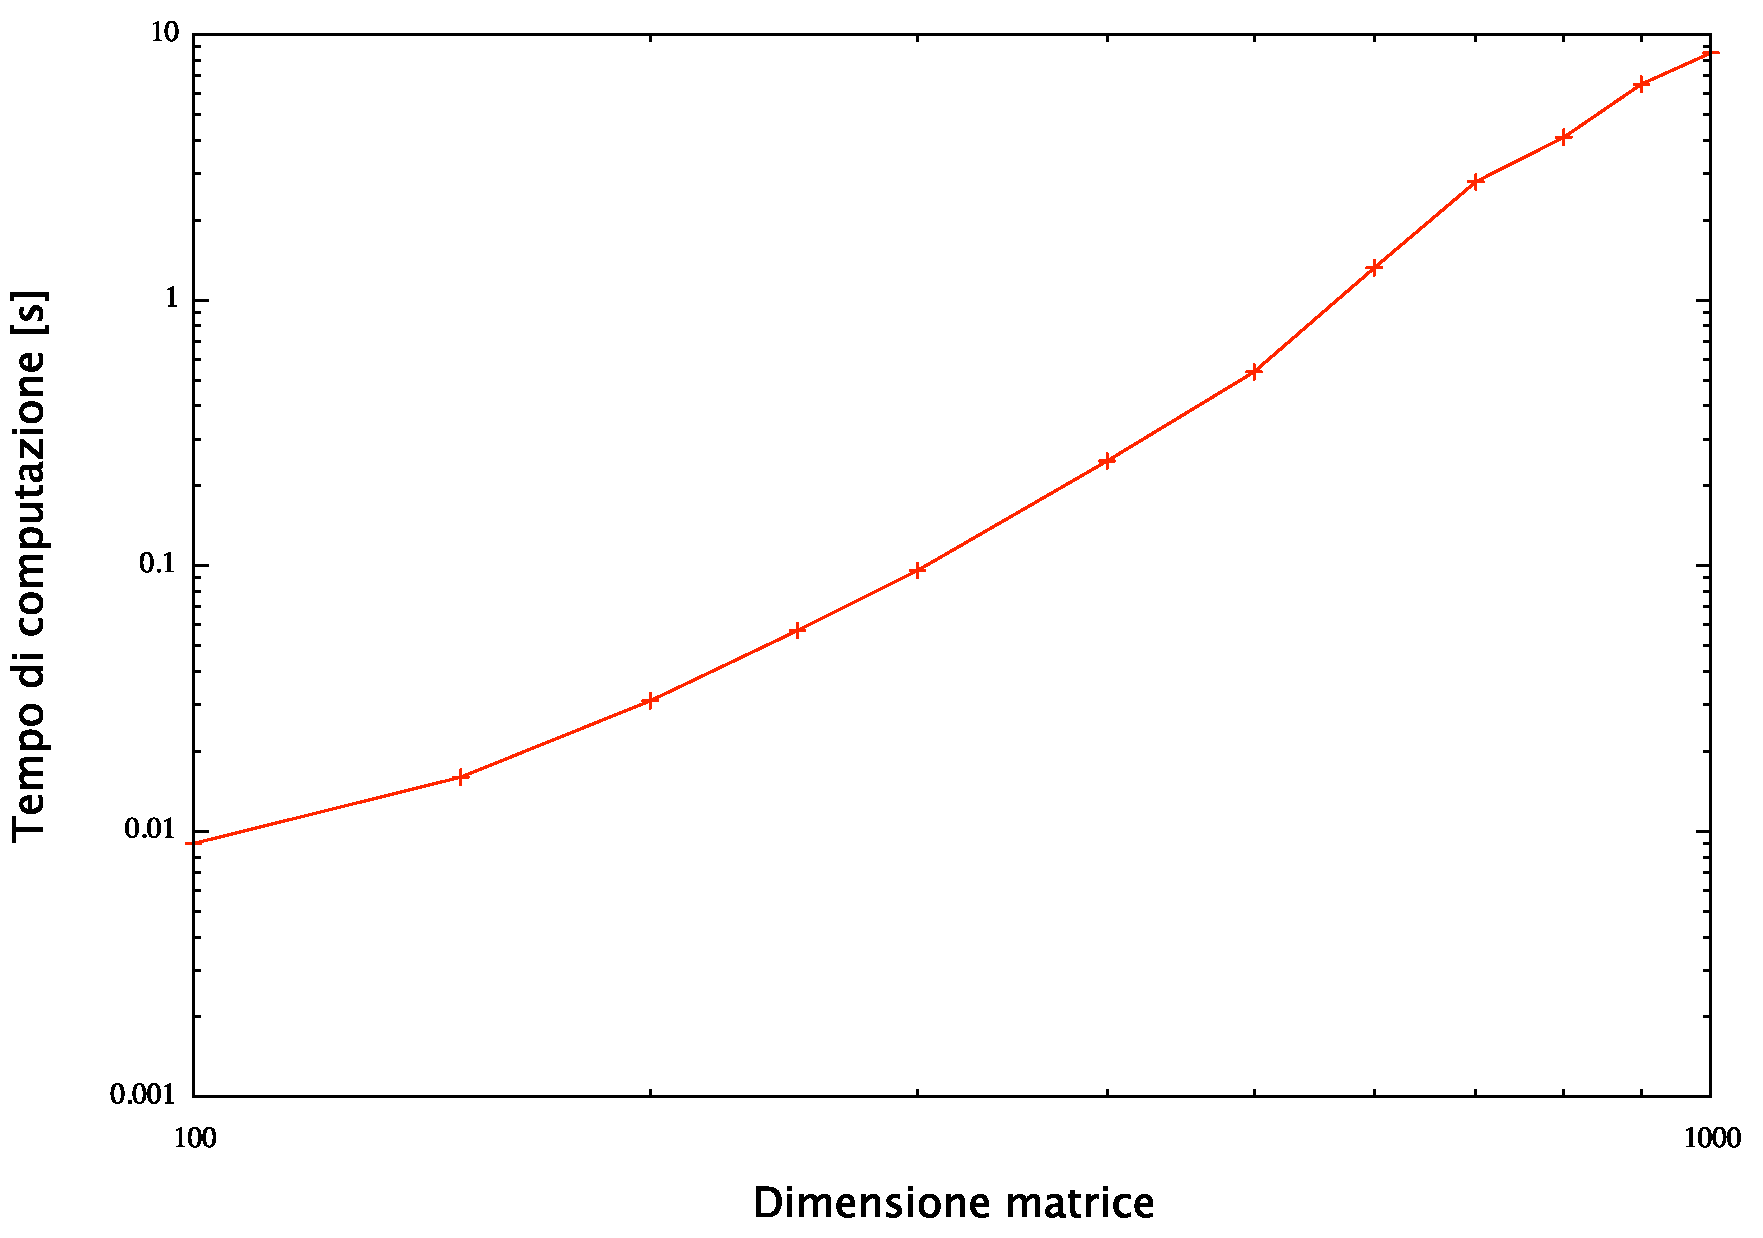
\includegraphics[scale=0.24]{dim-t}}
%\hspace{5mm}
%\subfigure[Convergenza di alcuni autovalori al risultato analitico in funzione della dimensione della matrice]
%{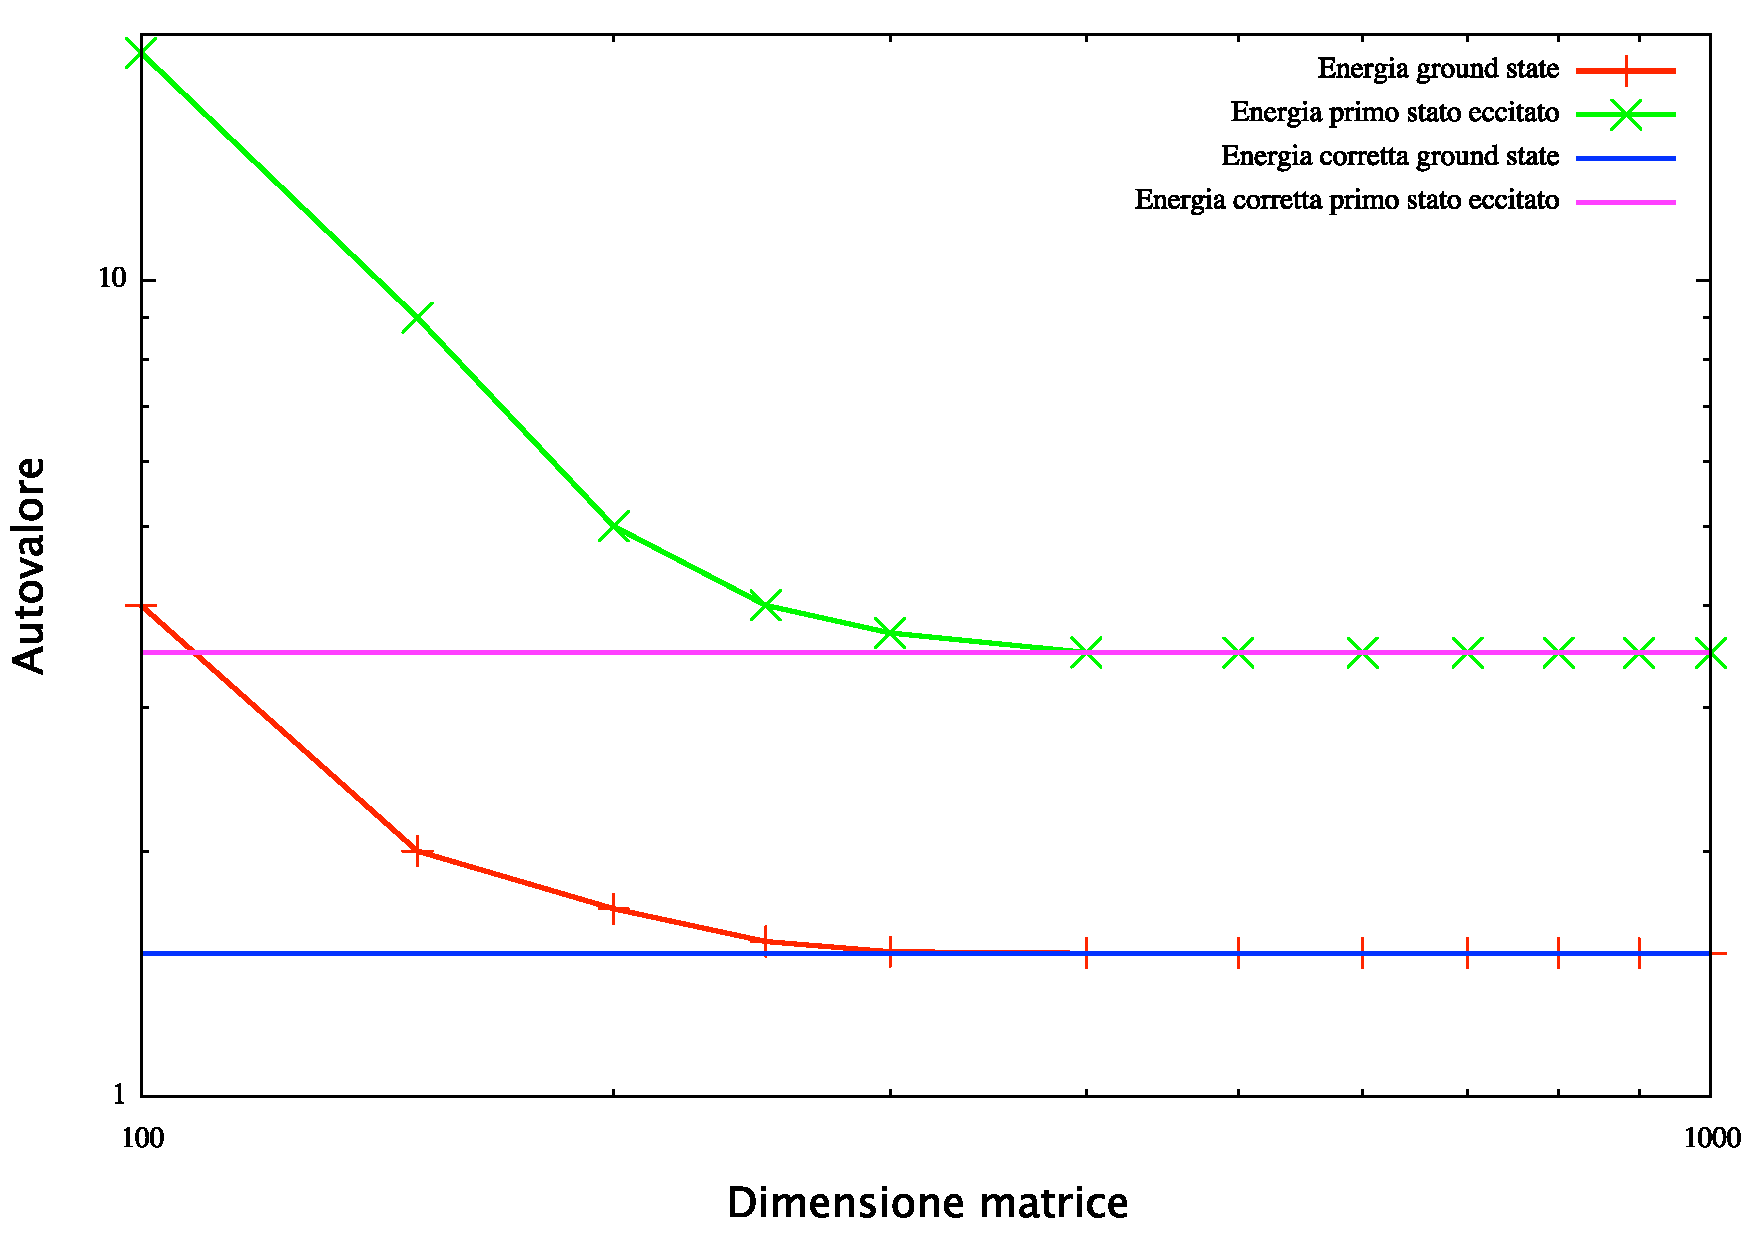
\includegraphics[scale=0.24]{conv-aut}}
%\end{figure}
%Com'è possibile vedere dal grafico, il valore per cui sia l'autovalore del ground state che quello del primo stato eccitato convergono al risultato analitico corrisponde a $D = 500$, dimensione che richiede un tempo di computazione intermedio. Cosa possiamo dire a riguardo dell'autostato? Sappiamo che il metodo con cui risolviamo l'equazione di Schr\"{o}dinger è preciso all'ordine $\Delta x$: possiamo inoltre supporre che, scelta la dimensione adeguata della matrice, l'errore indotto su $\psi(x)$ dal processo di diagonalizzazione $E_D$ risulti trascurabile rispetto a $\Delta x$: $E_D \ll \Delta x$. Siccome la soluzione analitica per $\psi(x)$ è nota, possiamo confrontare la soluzione ottenuta per il ground state con l'algoritmo di diagonalizzazione con $D=500$ e la soluzione analitica. In figura viene mostrata la differenza $\Delta \psi(x) = \psi_{analitica}(x) - \psi_{diag}(x)$. 
%\begin{figure}[!h]
%\centering
%\subfigure[Differenza $\Delta \psi(x)$]
%{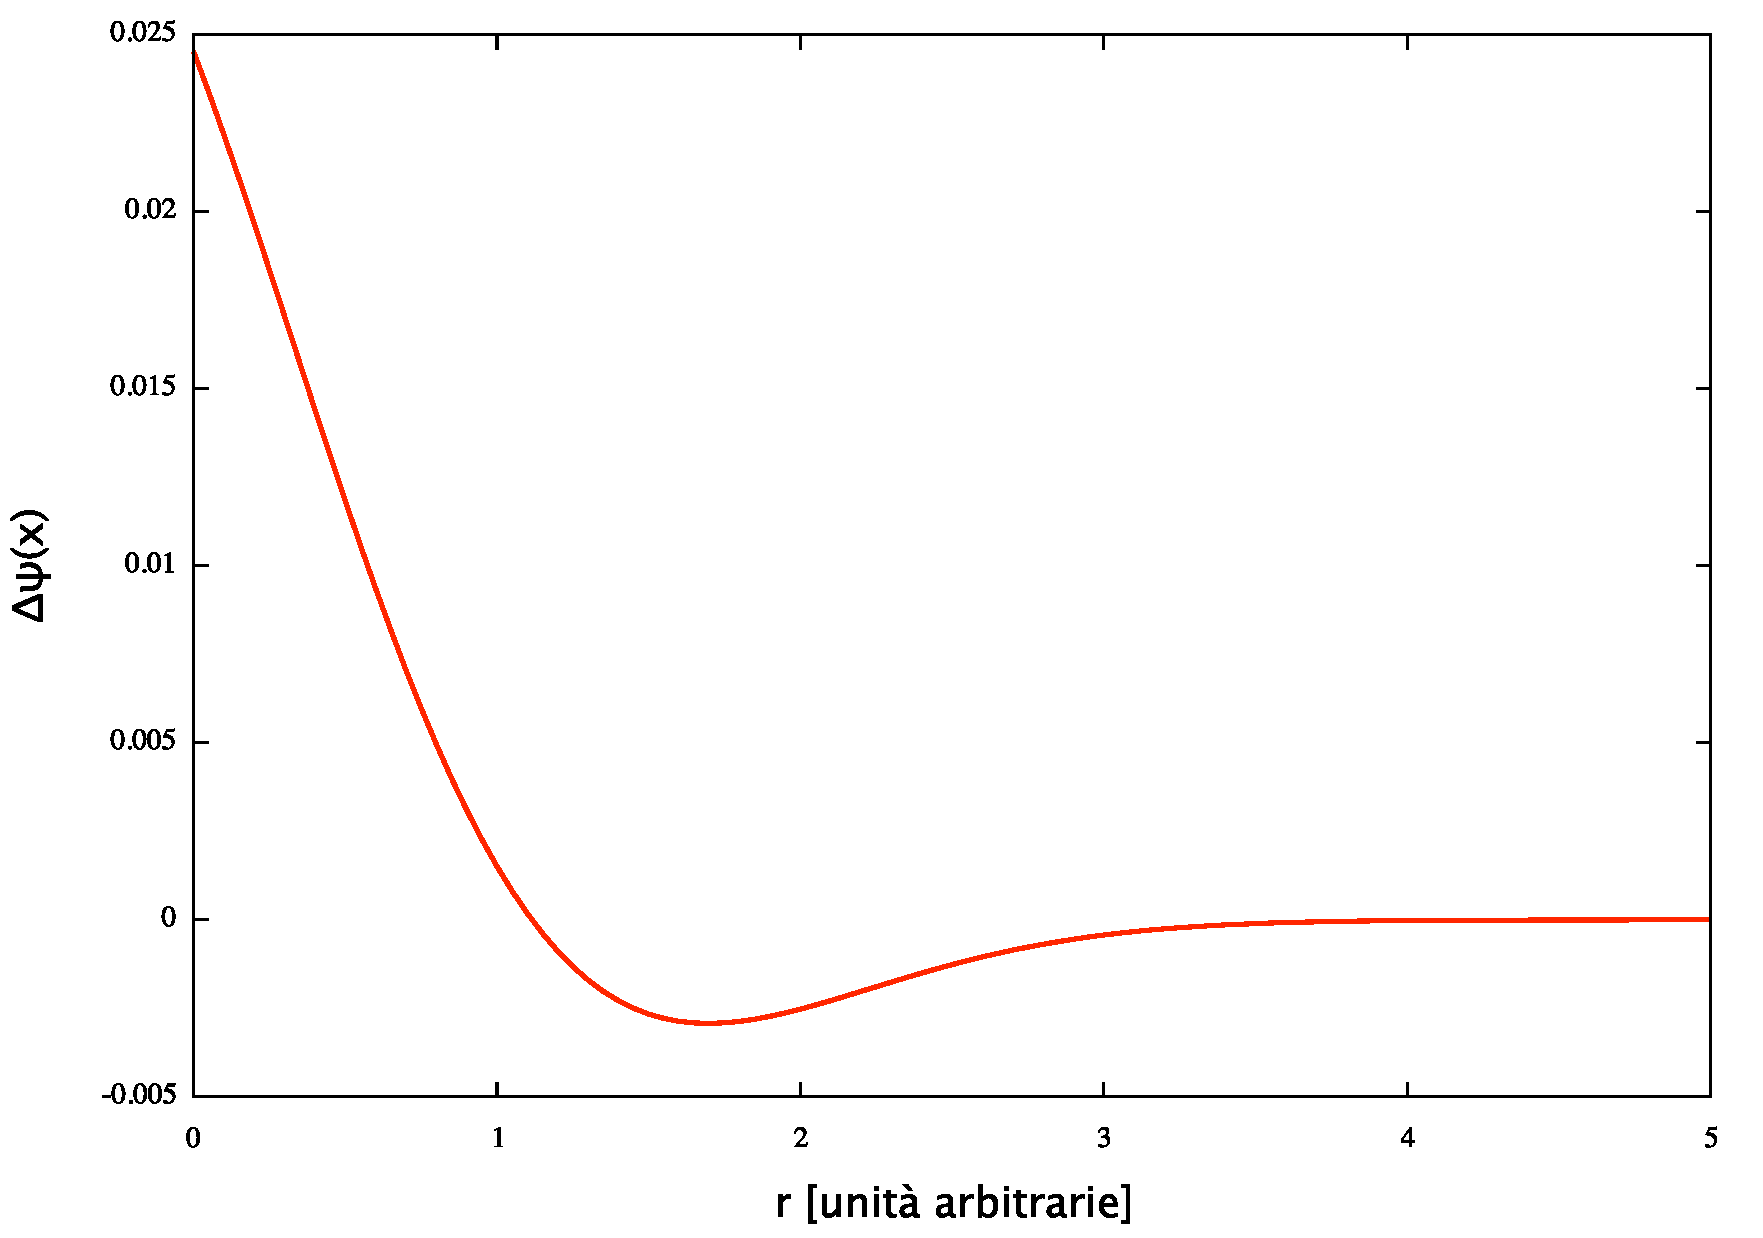
\includegraphics[scale=0.3]{deltapsi}}
%\end{figure}
%Si può notare come, essendo la precisione della soluzione $\Delta x = 0.05$, la differenza tra le due curve non superi mai la soglia imposta dall'incertezza. Conseguentemente, per il proseguo dell'analisi, $D=500$ verrà considerata la dimensione ideale per risolvere l'equazione di Schr\"{o}dinger con il metodo della diagonalizzazione. 
\subsection{Autoconsistenza}
Come si può evincere dall'equazione (6), il potenziale di Hartree dipende non solo dalla soluzione dell'equazione di singola particella, ma anche dalla soluzione di quelle di tutti gli altri fermioni nel sistema. Di conseguenza, l'algoritmo utilizzato per la risoluzione delle equazioni di Kohn-Sham è il seguente:
\begin{enumerate}[i.]
\item \textbf{Primo step}: fissare una densità \emph{guess} che funga da soluzione di prova per il calcolo del potenziale efficace. In questo caso, come densità guess si può scegliere una funzione che ricordi la distribuzione di Fermi, ovvero la distribuzione che rappresenta il numero medio di occupazione di un sistema di fermioni non interagenti:
\begin{equation}\label{17}
\rho(r) = \frac{1}{A} \frac{\rho_+}{1+e^{(r-R_c)}}
\end{equation}
dove il parametro $A$ viene fissato tramite la normalizzazione
\[
N = \int d^3r \rho(r)
\]
($\rho_+$ è un parametro di per sè ridondante che può essere incluso nella costante di normalizzazione). 
\item \textbf{Secondo step}: calcolare il potenziale efficace
\[
V_{eff}(r) = V_{ext}(r)+V_{int}(r) + \frac{\partial \varepsilon_{xc}}{\partial \rho}\rho + \varepsilon_{xc}
\]
\item \textbf{Terzo step}: risolvere le equazioni di Kohn-Sham per gli stati di singola particella attraverso l'algoritmo di diagonalizzazione: cioè ottenere $\varphi_i$ ed $\varepsilon_i$ per ogni stato occupato. Il numero di equazioni da risolvere dipende chiaramente dal numero di particelle nel sistema che, essendo fermioni, si distribuiranno in stati ad energie mano a mano più alte. Conseguentemente, è necessario risolvere le equazioni per tutti i momenti angolari che potrebbero entrare in gioco, e successivamente ordinare gli autovalori in maniera da fissare l'ordine di occupazione degli orbitali. 
\item \textbf{Terzo step}: calcolare la nuova densità del sistema, ottenuta come
\begin{equation}
\rho_{new}(r) = \sum_{\text{stati occupati}} d_i|\varphi_i(r)|^2
\end{equation}
dove $d_i$ è la degenerazioni dello stato $i$-esimo. Per evitare di incorrere in soluzioni metastabili che impediscano la convergenza è possibile a questo punto scegliere un parametro di ''ammorbidimento'' $\alpha < 1$ adeguatamente piccolo (verrà discussa in seguito la scelta del suo valore), e definire
\begin{equation}
\rho_{new}^{(1)}(r) = \alpha \rho_{new}(r) + (1-\alpha)\rho_{old}(r)
\end{equation}
(dove, nel caso della prima iterazione $\rho_{old} \equiv \rho_{guess}$) utilizzandolo per calcolare la somma degli autovalori $\varepsilon_i$: $\sum_{\text{stati occupati}} \varepsilon_i^{(1)}$.
\item \textbf{Quarto step}: verificare la condizione di uscita
\begin{equation}
\left| \sum_{i=1}^N \varepsilon_i^{(k)} - \sum_{i=1}^N \varepsilon_i^{(k-1)} \right| < \varepsilon
\end{equation}
ovvero verificare se la somma degli autovalori al ciclo k-esimo è uguale, a meno di un $\varepsilon$ fissato, a quella del ciclo precedente. Se questa condizione è soddisfatta, l'iterazione cessa e si considera raggiunta la convergenza. 
\end{enumerate}

\section{Risultati}
\subsection{Unità ridotte}
Sono state scelte le seguenti unità per la soluzione delle equazioni: 
\[
m = \hbar = e = 1 \qquad a_0 = 0.53 \overset{\circ}{A}
\]
dove $a_0$ è il \emph{raggio di Bohr}. In queste unità, l'energia viene calcolata in \emph{Hartree} ($H$): in eV abbiamo la conversione
\begin{equation}
1 H = \frac{\hbar^2}{m_e a_0^2} \ \text{eV} = 27,21 \text{eV}
\end{equation}  
\subsection{Informazioni generali sul software}

L'esecuzione del programma richiede a scelta di certi parametri (cfr. Autoconsistenza):
\begin{itemize}
\item $r_s$: il raggio di Wiegner-Seitz è stato posto convenzionalmente pari a $r_s=4$ in unità del raggio di Bohr (il valore corrispondente al sodio);
	\item $R_{max}$: tale parametro rappresenta la lunghezza della griglia numerica scelta per la soluzione del problema. In questo caso, dopo una serie di test preliminari si è scelto $R_{max} = 20$;
	\item $\Delta x$: fissata la lunghezza della mesh, per ottenere una matrice sufficientemente grande da garantire una diagonalizzazione significativa è stato scelto $\Delta x = 0.015$;
	\item $\alpha$: il valore di $\alpha$ è stato settato, dopo alcuni test preliminari di convergenza, a $\alpha=0.05$;
	\item $\varepsilon$: questo parametro fissa la sensibilità sulla convergenza dell'algoritmo e dunque è necessario settarlo in maniera tale da non sovrastimare la precisione del processo computazionale ma contemporaneamente da garantire una convergenza ad un valore sufficientemente stabile. In questo particolare caso è stato scelto $\varepsilon = 10^{-3}$. 
\end{itemize}
\subsection{Discussione dei risultati}
In questo paragrafo verranno mostrati i risultati ottenuti tramite il metodo precedentemente descritto. Cominciamo con le energie del sistema $E[\rho]$ per differenti configurazioni closed-shell:
\begin{center}
\begin{tabular}{|c|c|c|c|}
\hline
$N_{fermioni}$ & \emph{Orbitali occupati} & $E[\rho]/N$ $[$H$]$ & $E[\rho]/N$ $[$eV$]$ \\ \hline
2 & 1s & -0.308 $\pm$ 0.001 & -8.37 $\pm$ 0.01 \\ \hline
8 & 1s, 1p & -0.675 $\pm$ 0.001 & -18.38 $\pm$ 0.01 \\ \hline
18 & 1s, 1p, 1d & -1.052 $\pm$ 0.001 & -28.63 $\pm$ 0.01 \\ \hline
20 & 1s, 1p, 1d, 2s & -1.174 $\pm$ 0.001 & -31.94 $\pm$ 0.01 \\ \hline
34 & 1s, 1p, 1d, 2s, 1f & -1.653 $\pm$ 0.001 & -44.97 $\pm$ 0.01 \\ \hline
40 & 1s, 1p, 1d, 2s, 1f, 2p & -1.829 $\pm$ 0.001 & -49.78 $\pm$ 0.01 \\ \hline
\end{tabular}
\end{center}\ \\
Di seguito mostriamo invece i risultati per quanto riguarda la densità, il potenziale di Hartree ed il potenziale di scambio-correlazione ottenuti a convergenza. Tutti i plot mostrano le funzioni ottenute tramite la densità guess \eqref{17} e le conseguenti funzioni a convergenza. Per la densità:
\newpage
\begin{figure}[!h]
\centering
\subfigure[$N=2$]
{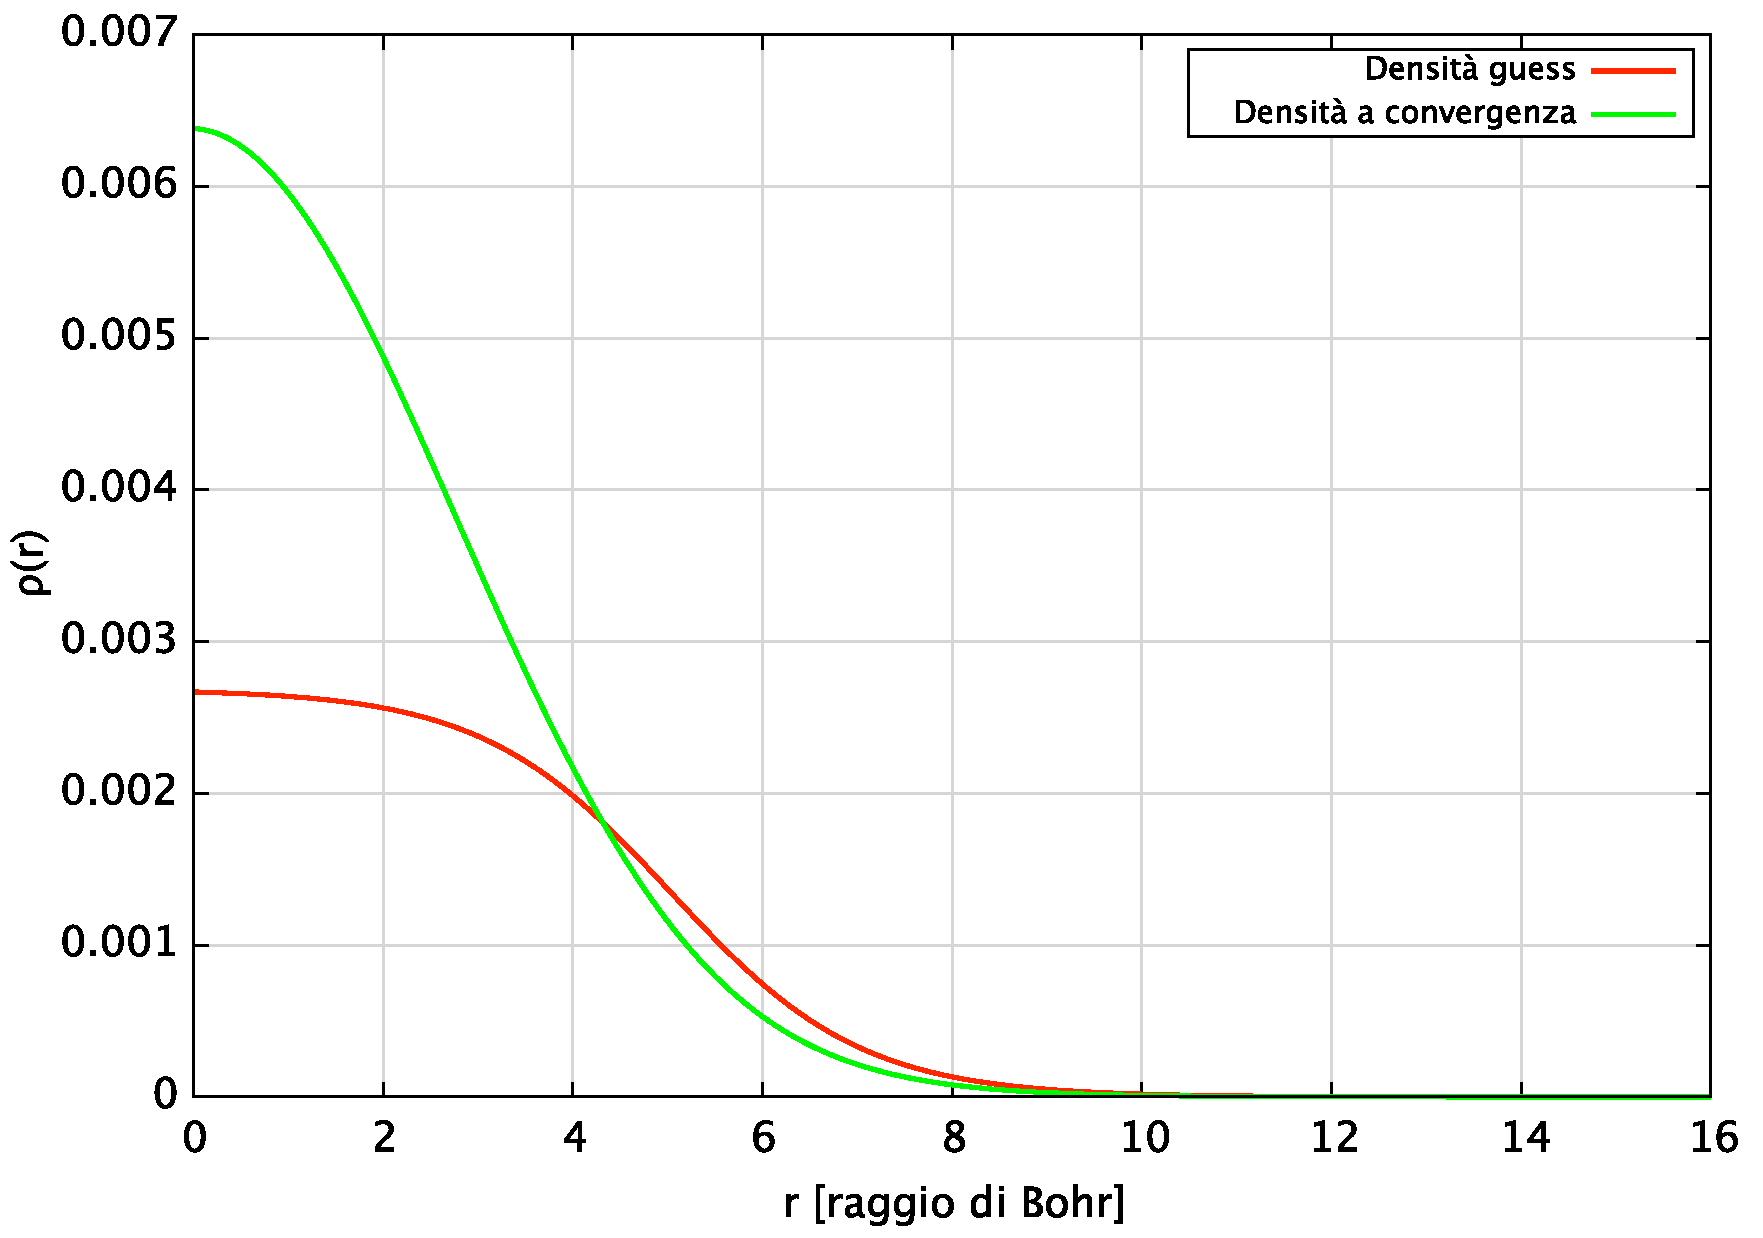
\includegraphics[scale=0.25]{Img/dens-2}}
\hspace{3mm}
\subfigure[$N=8$]
{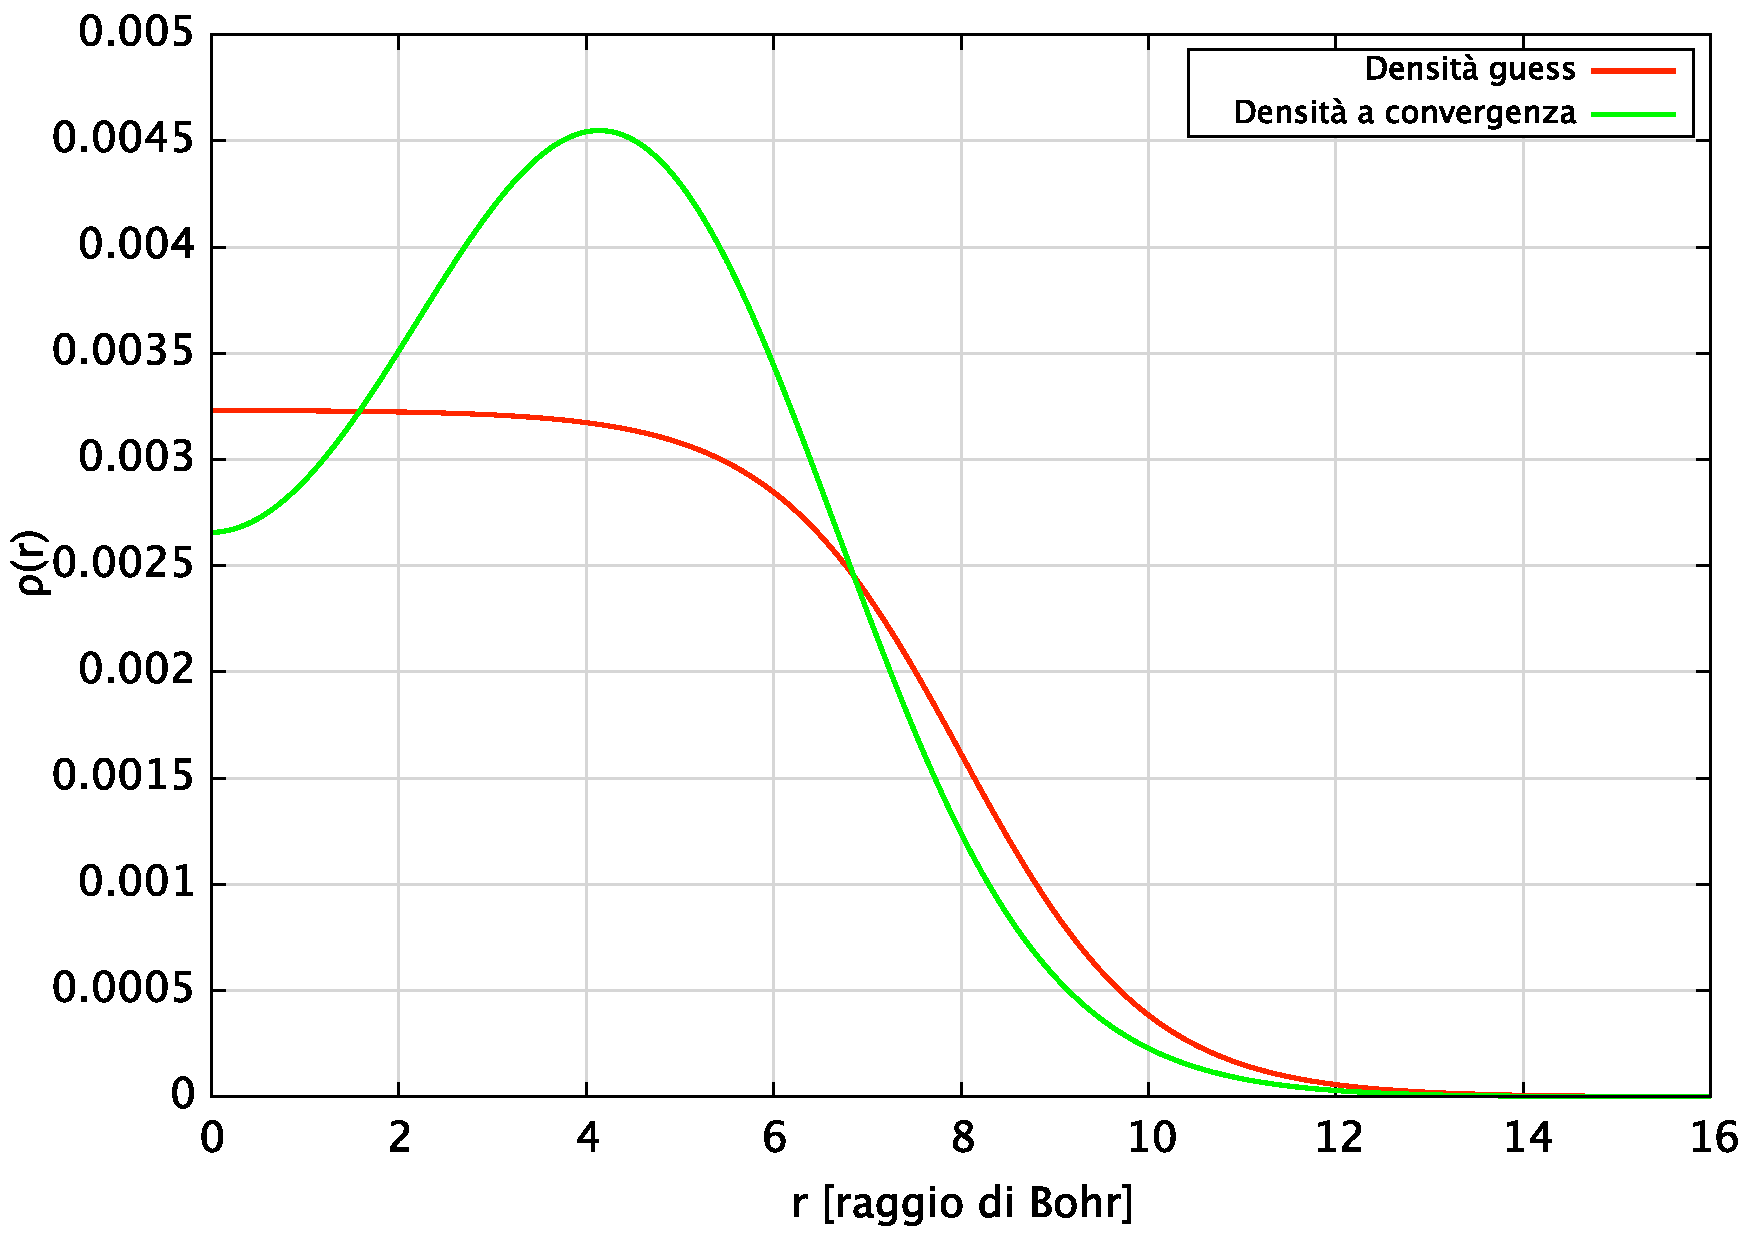
\includegraphics[scale=0.25]{Img/dens-8}}
\subfigure[$N=18$]
{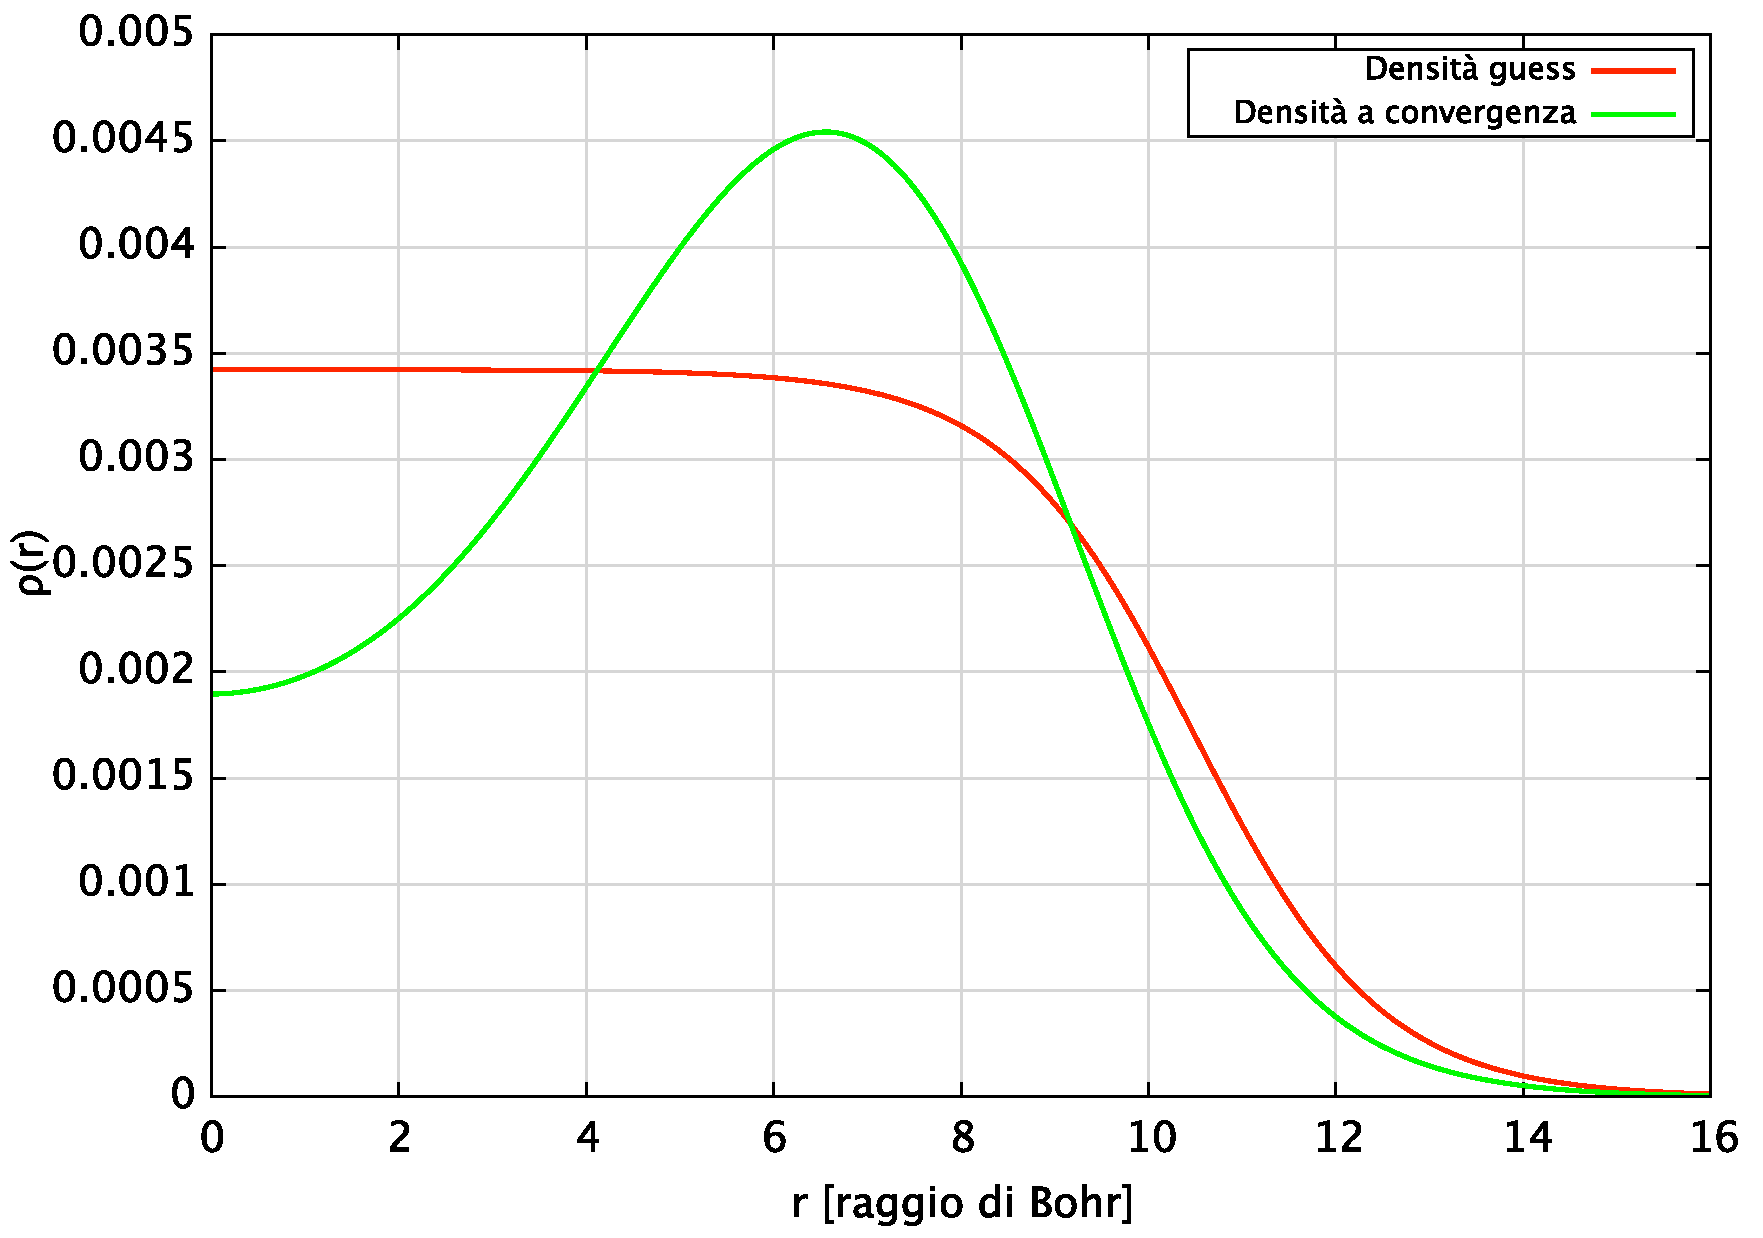
\includegraphics[scale=0.25]{Img/dens-18}}
\hspace{3mm}
\subfigure[$N=20$]
{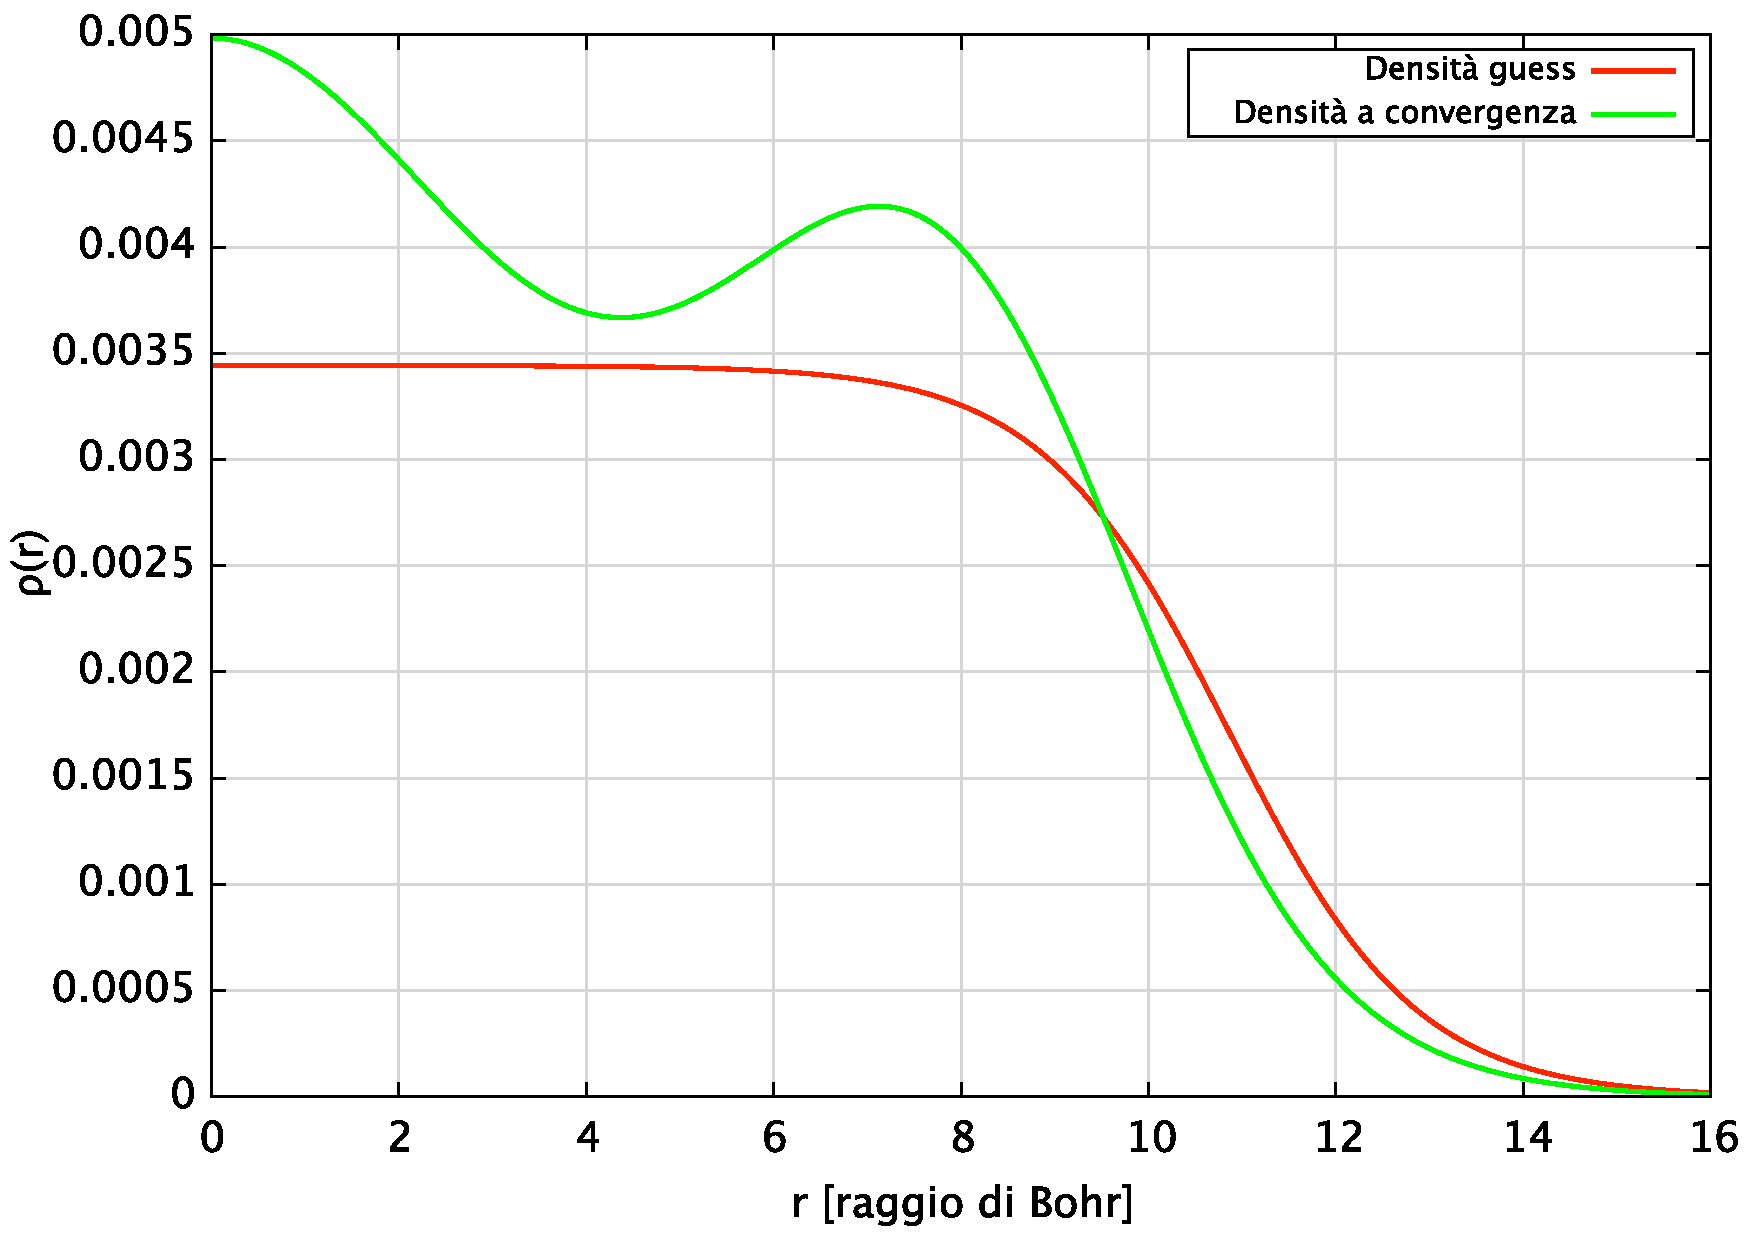
\includegraphics[scale=0.25]{Img/dens-20}}
\subfigure[$N=34$]
{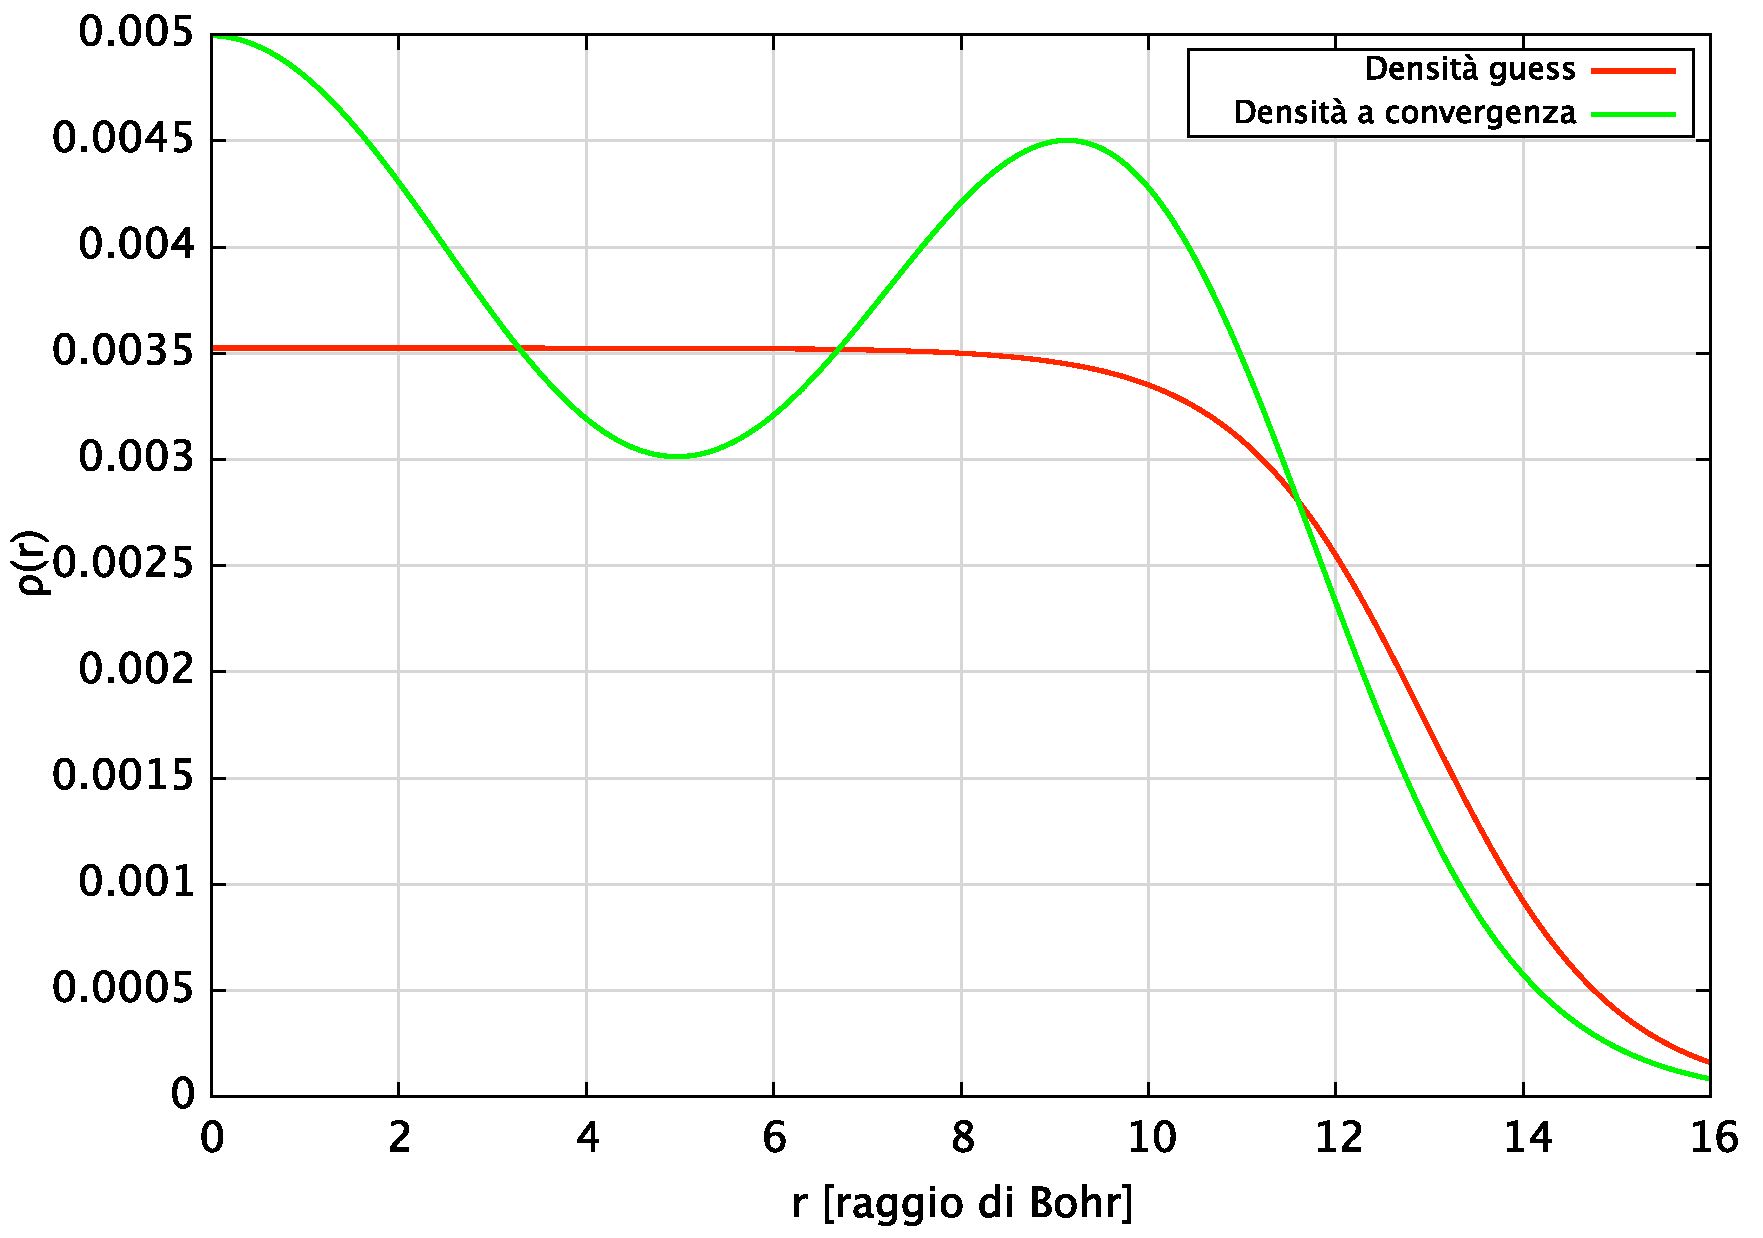
\includegraphics[scale=0.25]{Img/dens-34}}
\hspace{3mm}
\subfigure[$N=40$]
{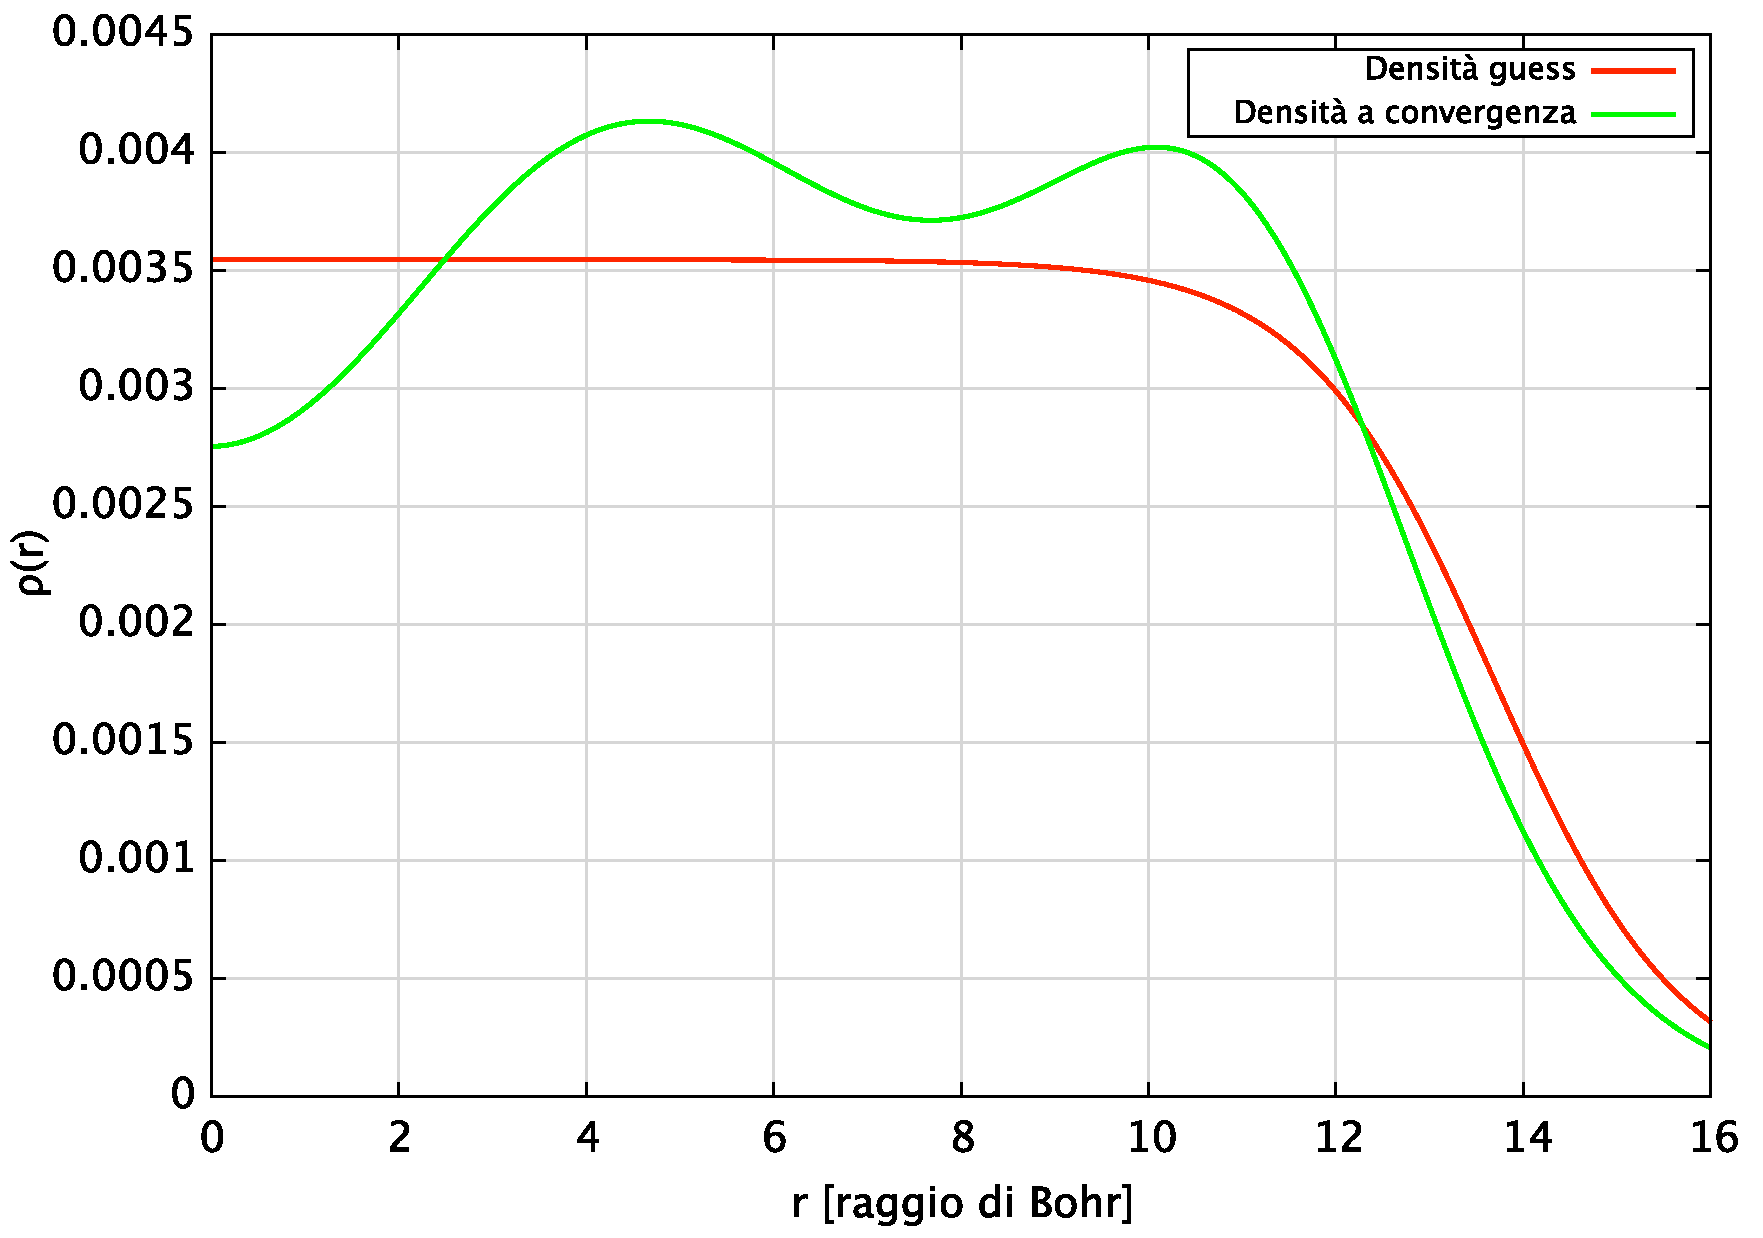
\includegraphics[scale=0.25]{Img/dens-40}}
\caption{Plot delle densità del sistema fermionico nelle diverse configurazioni a shell chiusa}
\end{figure}\ \\
Le densità rispecchiano le previsioni sul comportamento del sistema: nel caso di due soli fermioni il picco della densità è ovviamente in $r=0$, in quanto le due particelle sono in onda $s$. Aumentando il numero di shell a disposizione vediamo il massimo allontanarsi da zero attraverso il contributo degli orbitali $1p$ e $1d$ e così via fino alla conformazione più complessa che corrisponde a $N=40$, dove si sommano i contributi di sei differenti orbitali pesati con le rispettive degenerazioni. La figura (f) può essere confrontata con Fig. 2.4 di [1], evidenziando (almeno qualitativamente) un comportamento simile a quello della simulazione di riferimento. 
\newpage
\begin{figure}[!h]
\centering
\subfigure[$N=2$]
{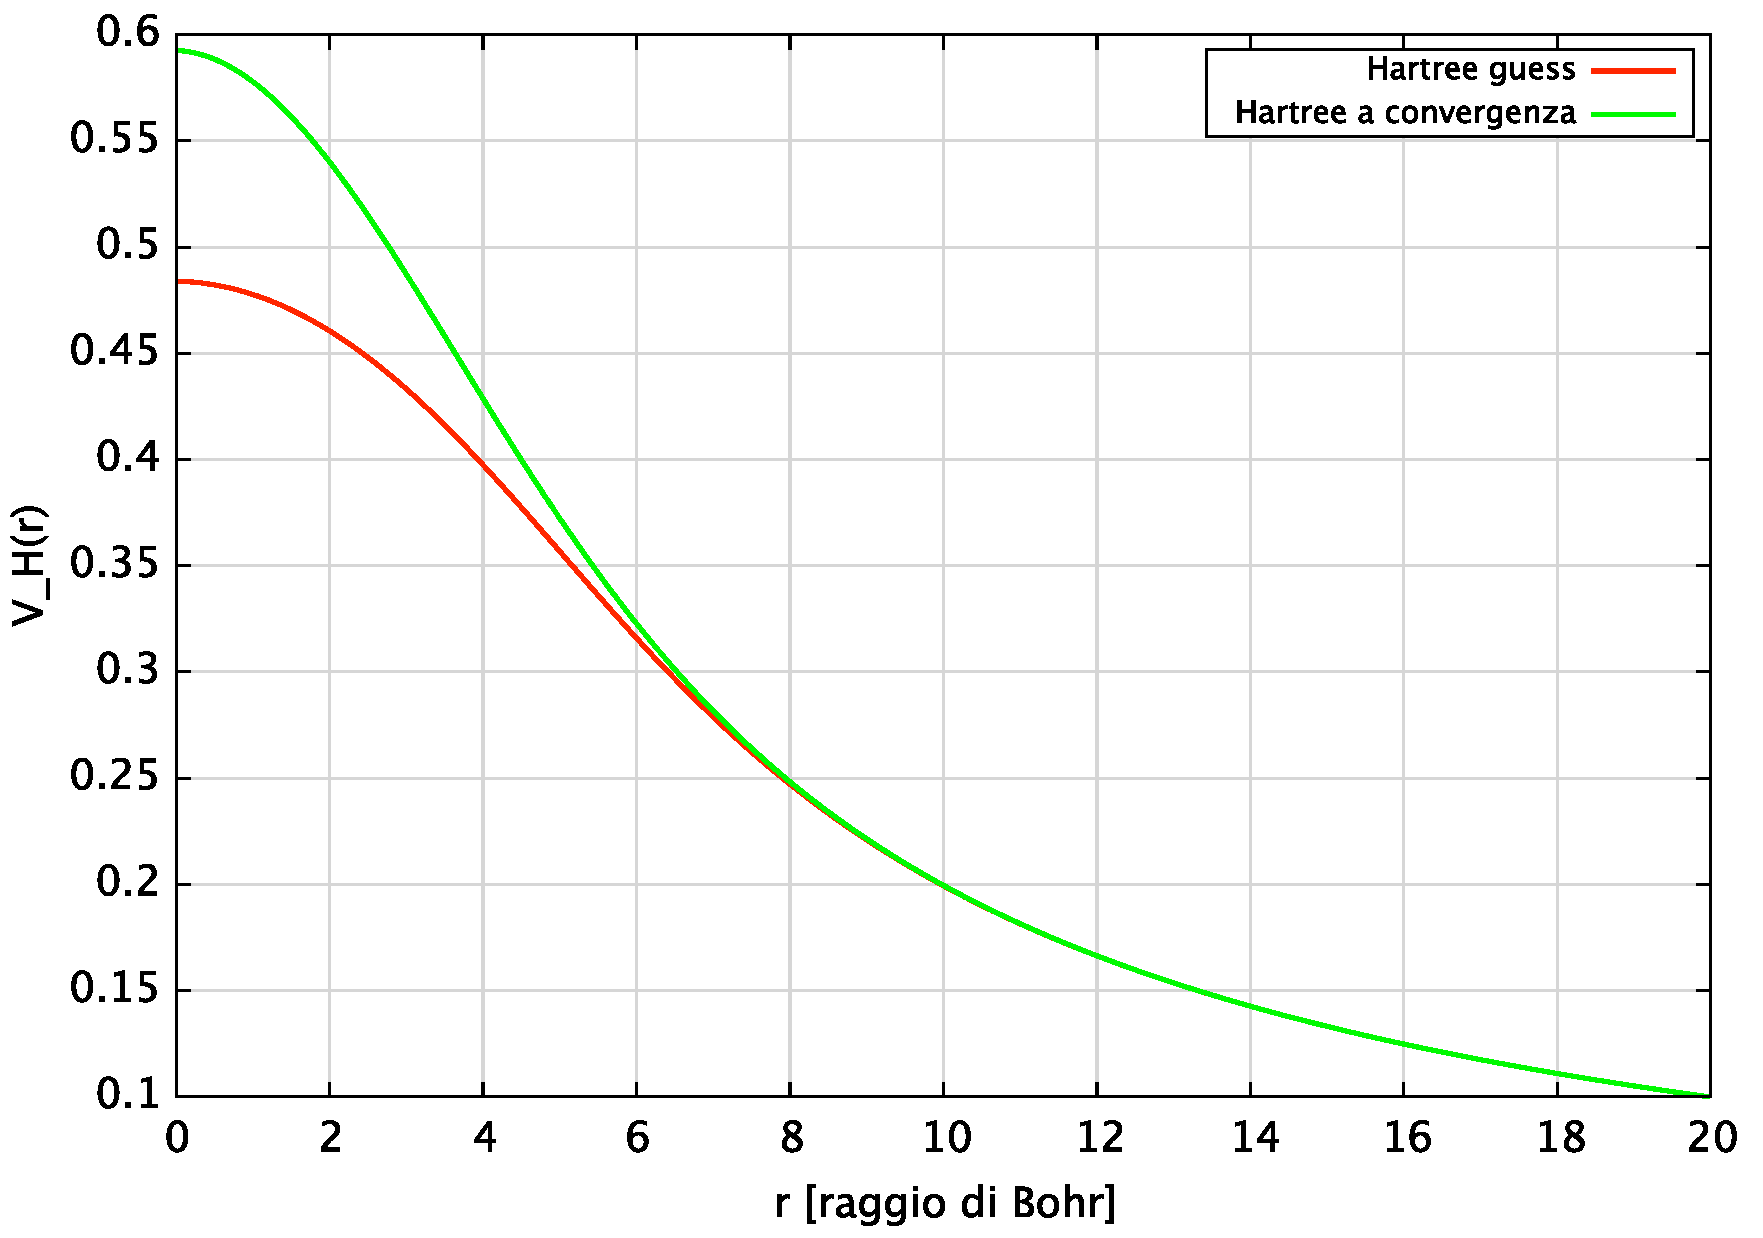
\includegraphics[scale=0.25]{Img/h-2}}
\hspace{3mm}
\subfigure[$N=8$]
{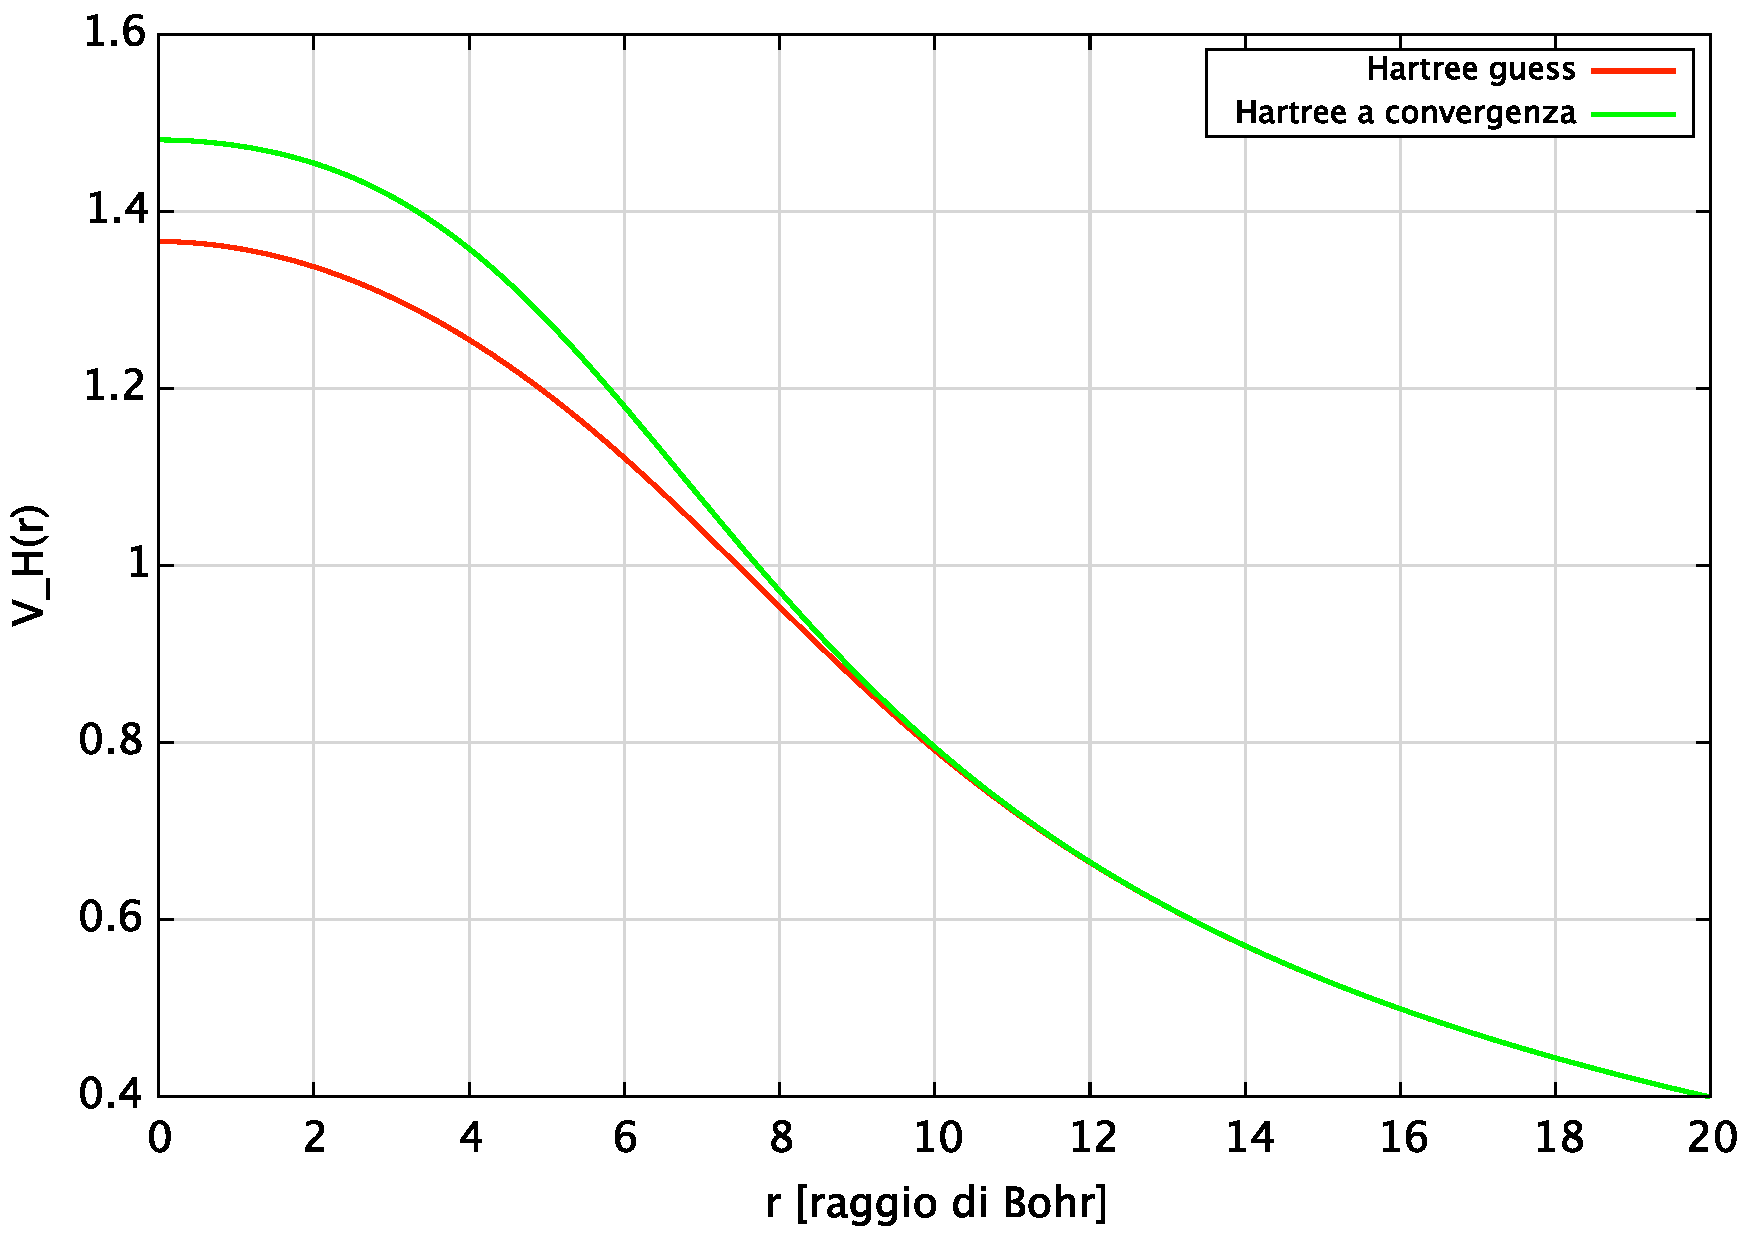
\includegraphics[scale=0.25]{Img/h-8}}
\subfigure[$N=18$]
{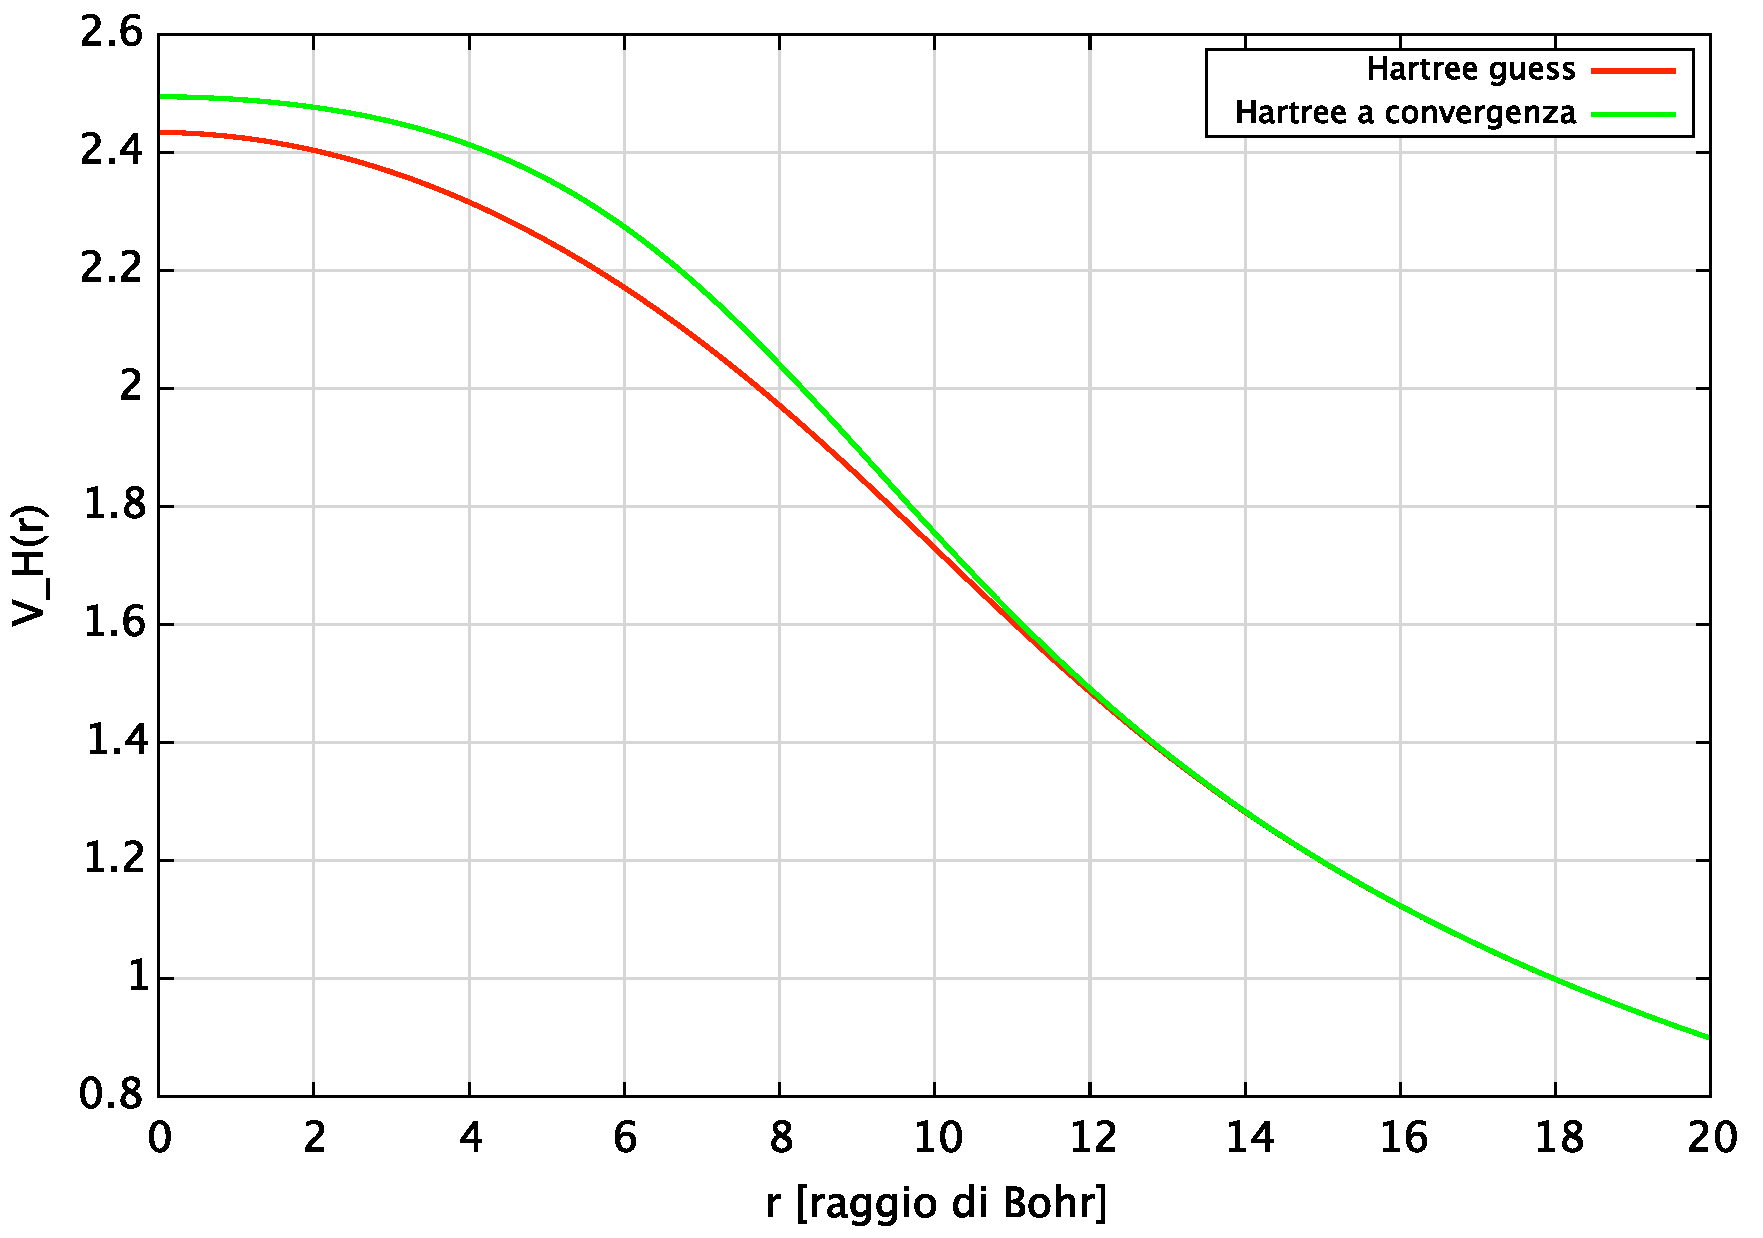
\includegraphics[scale=0.25]{Img/h-18}}
\hspace{3mm}
\subfigure[$N=20$]
{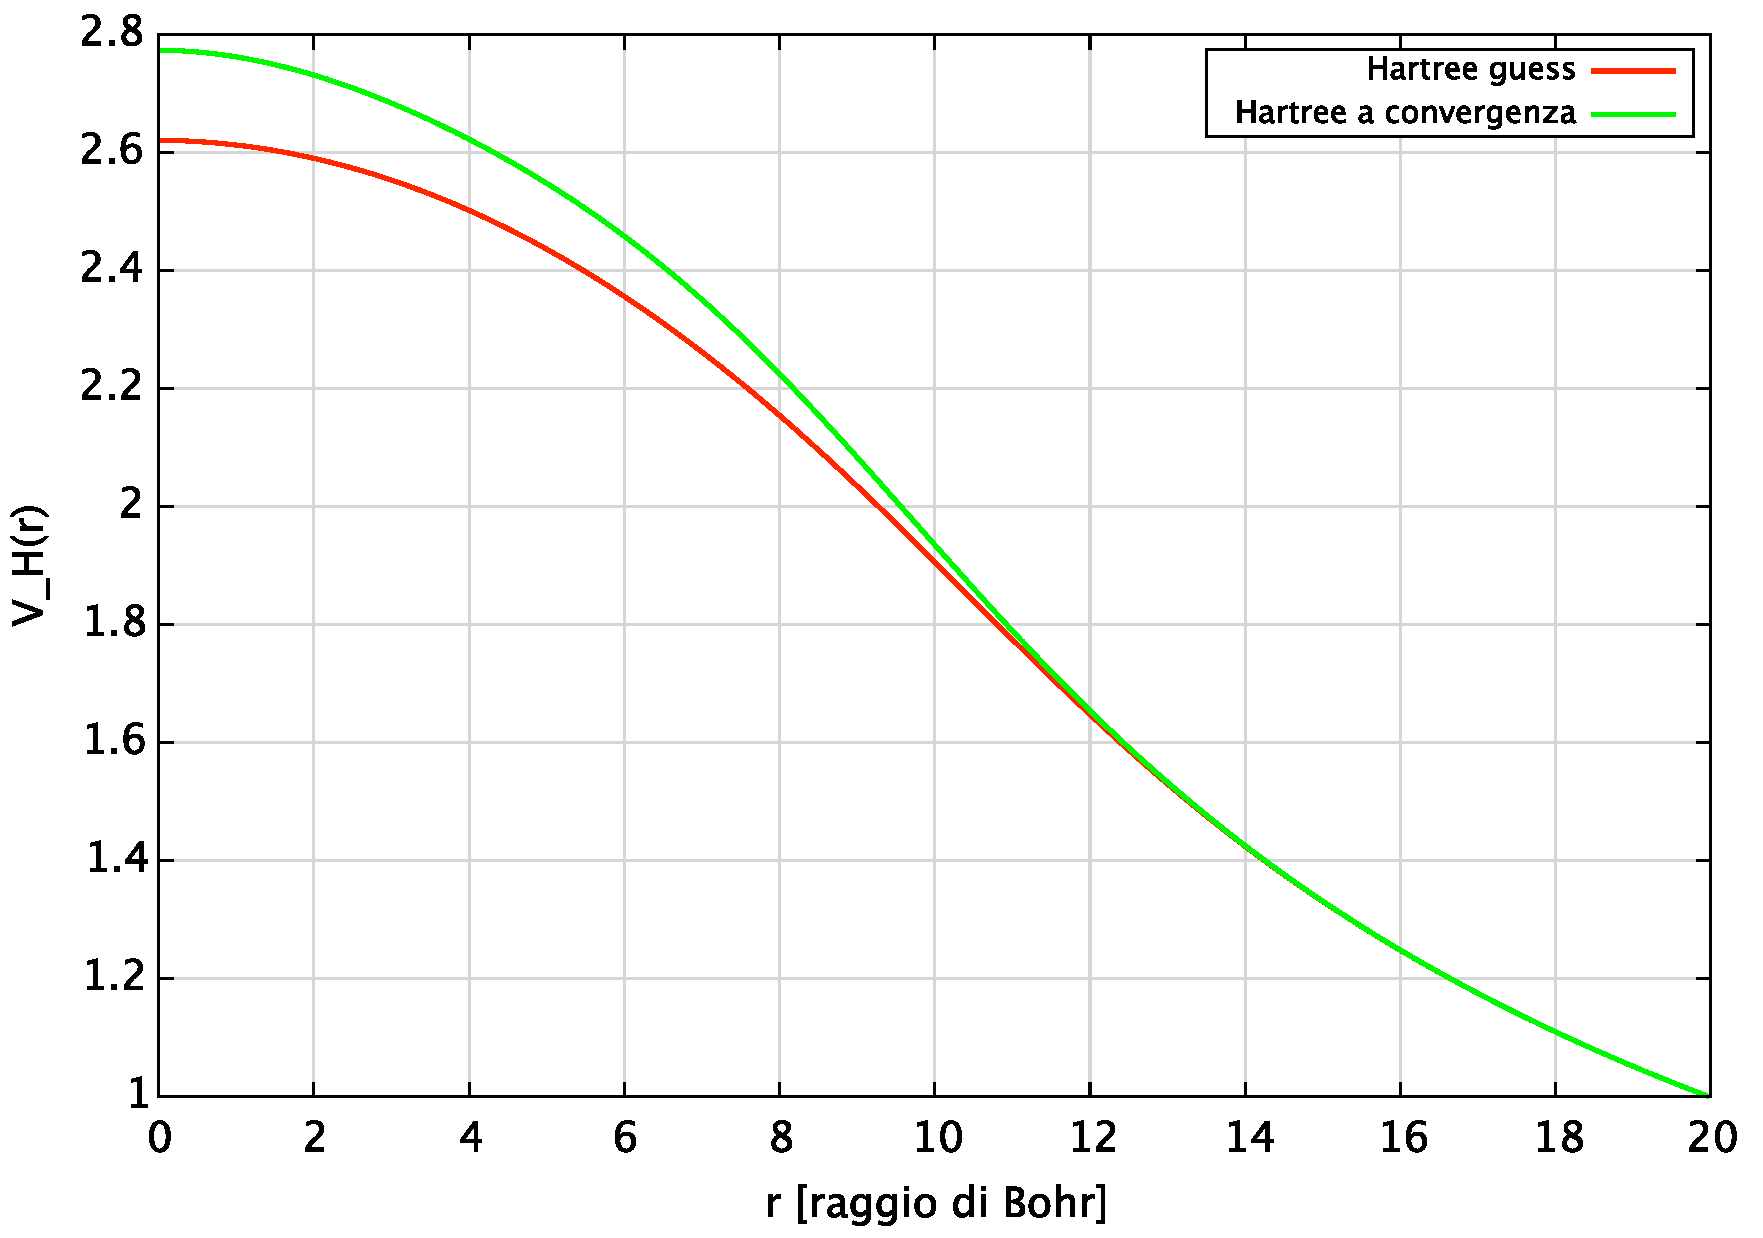
\includegraphics[scale=0.25]{Img/h-20}}
\subfigure[$N=34$]
{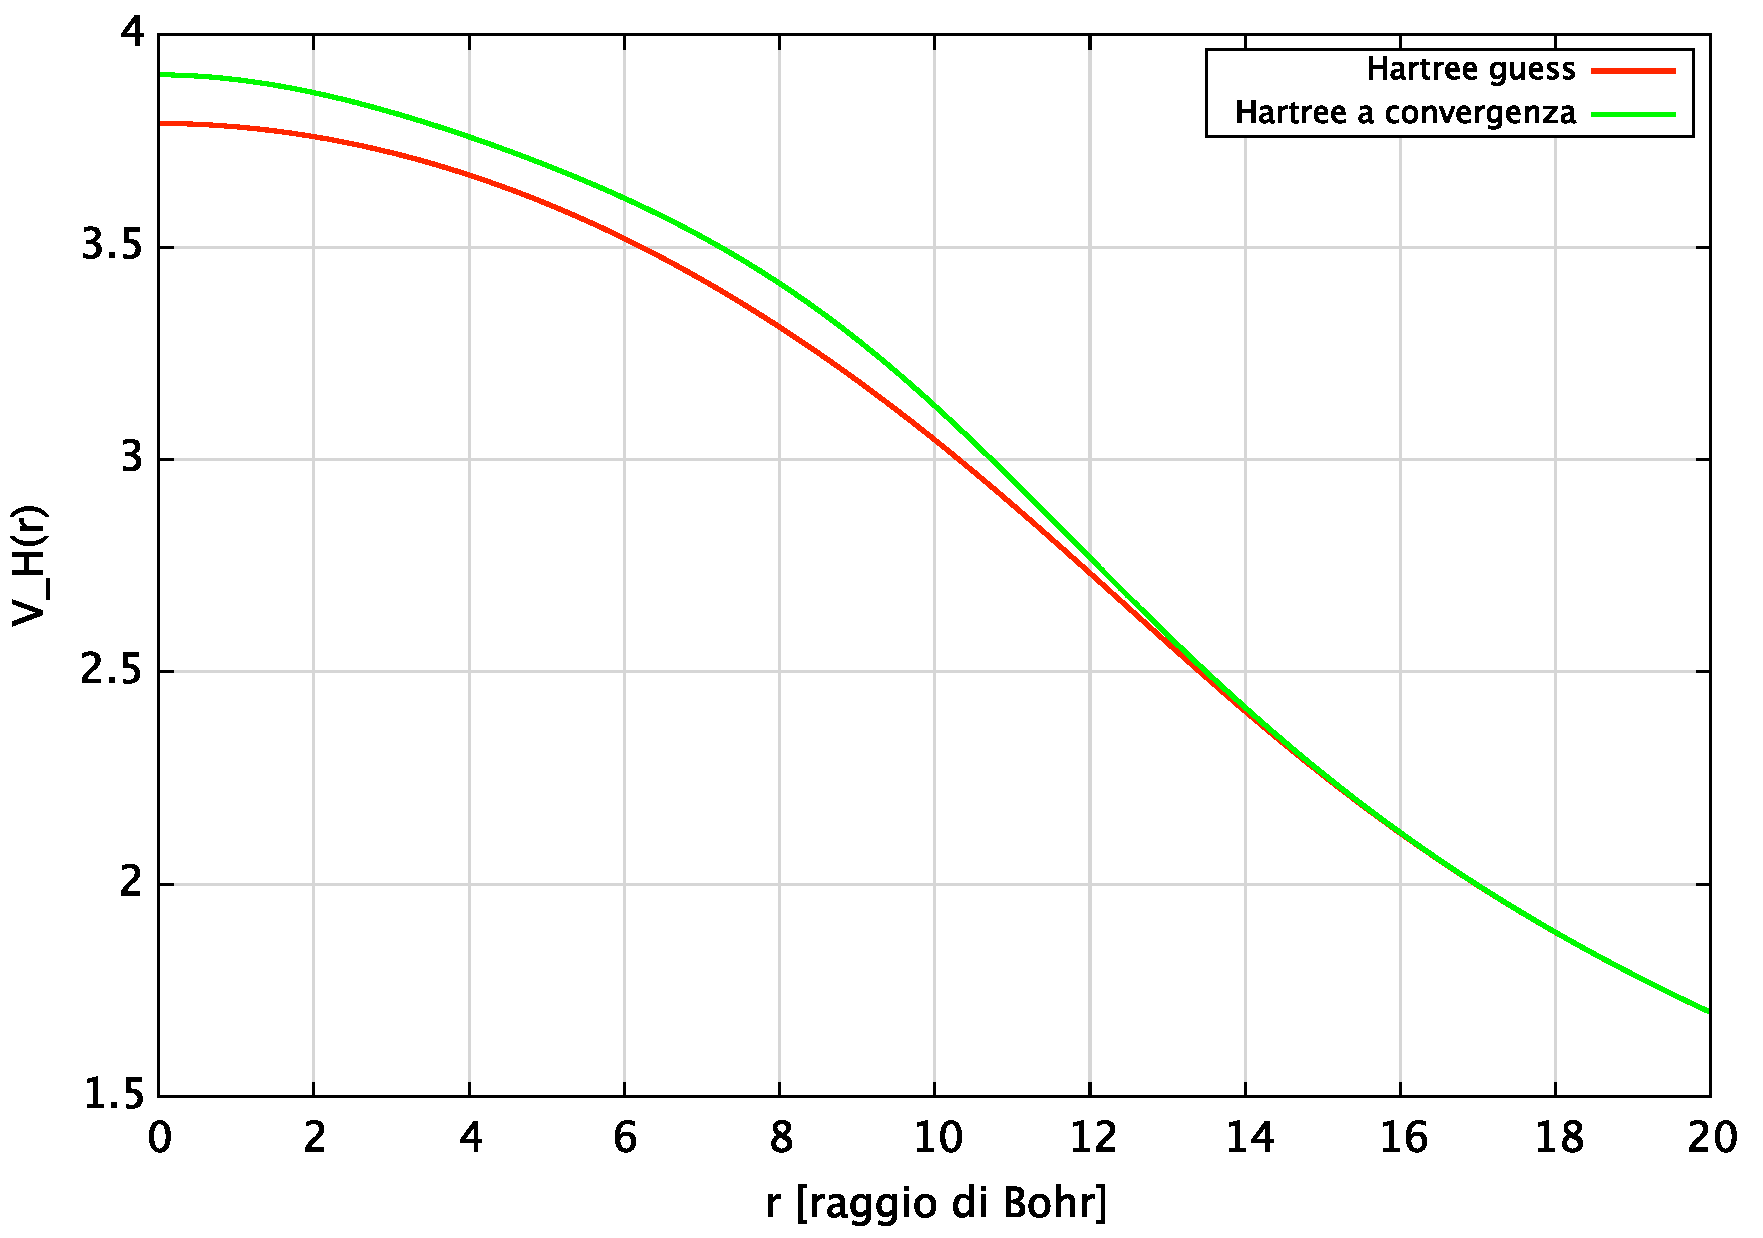
\includegraphics[scale=0.25]{Img/h-34}}
\hspace{3mm}
\subfigure[$N=40$]
{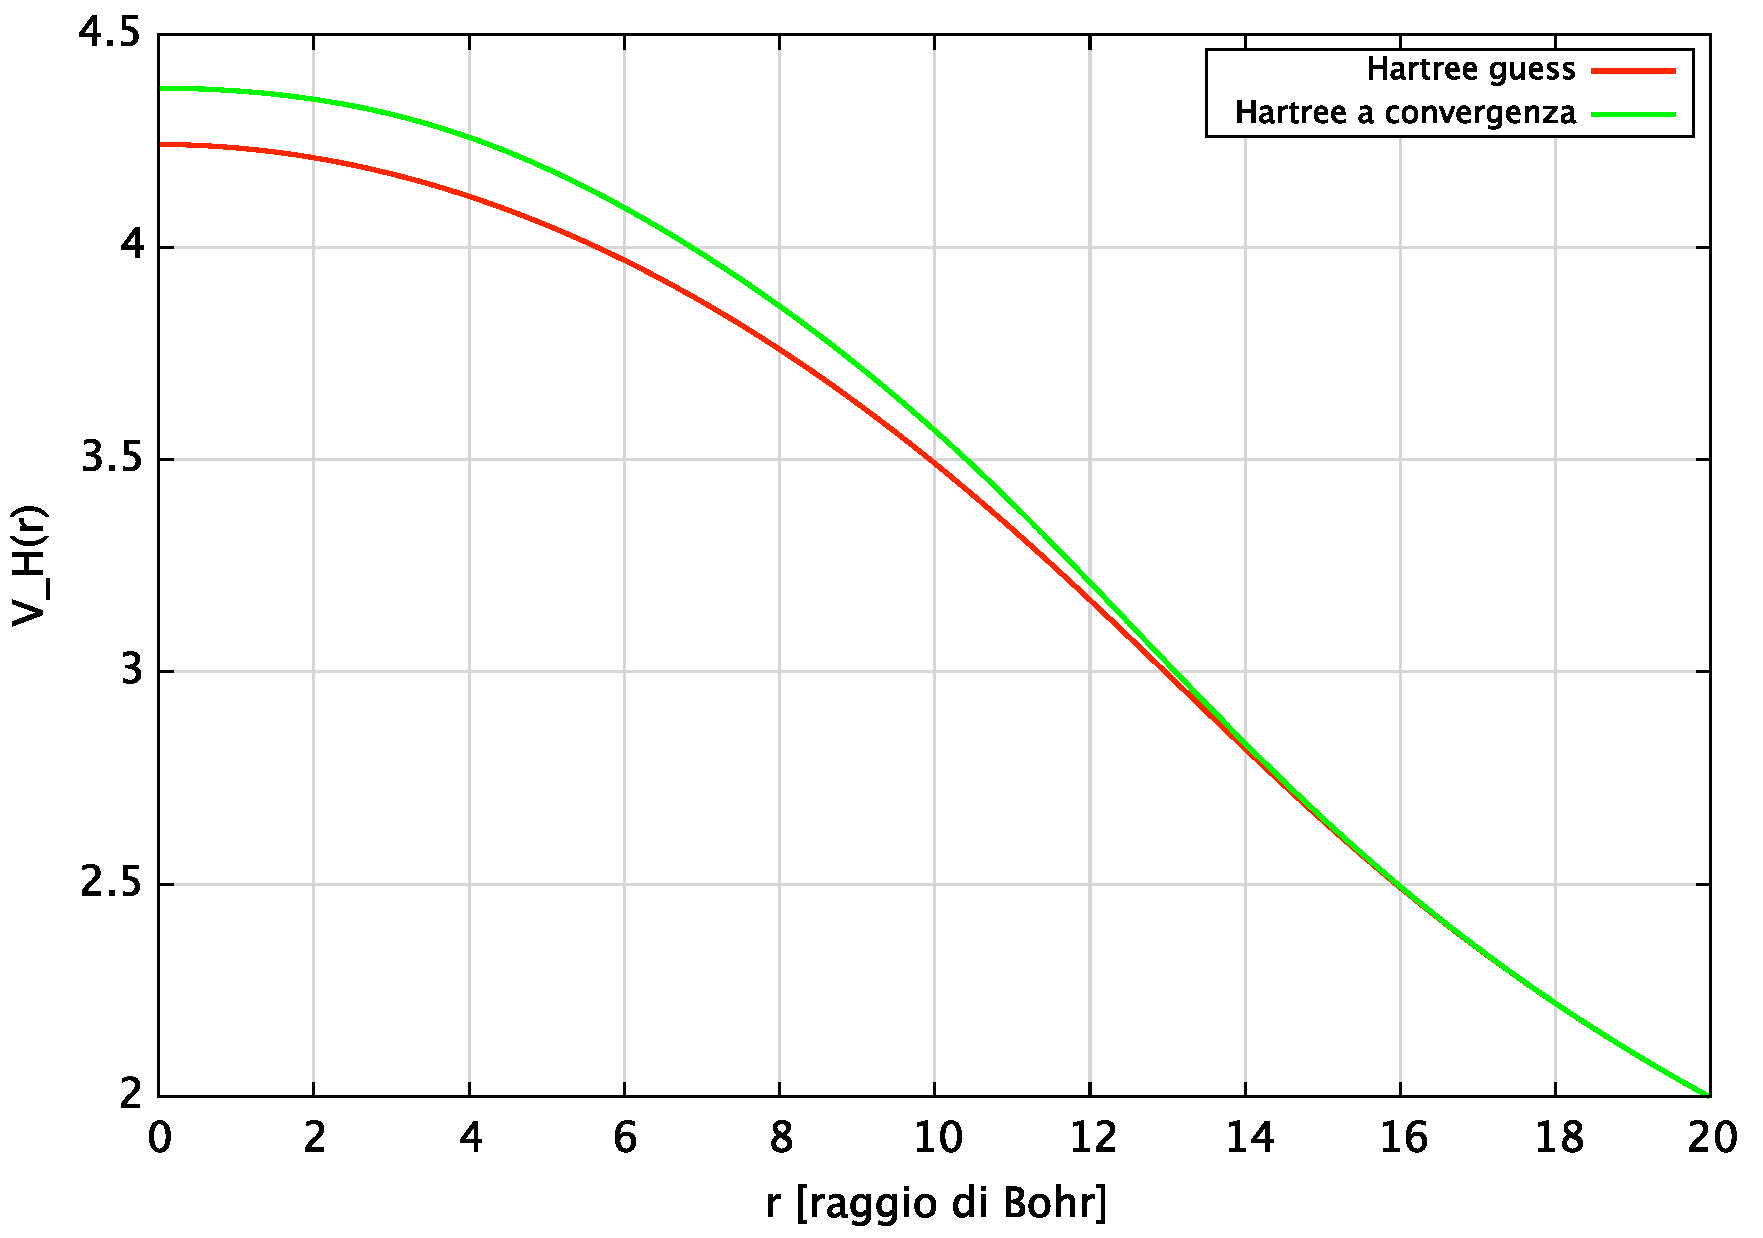
\includegraphics[scale=0.25]{Img/h-40}}
\caption{Plot del potenziale di Hartree del sistema fermionico nelle diverse configurazioni a shell chiusa}
\end{figure}\ \\
\newpage
\begin{figure}[!h]
\centering
\subfigure[$N=2$]
{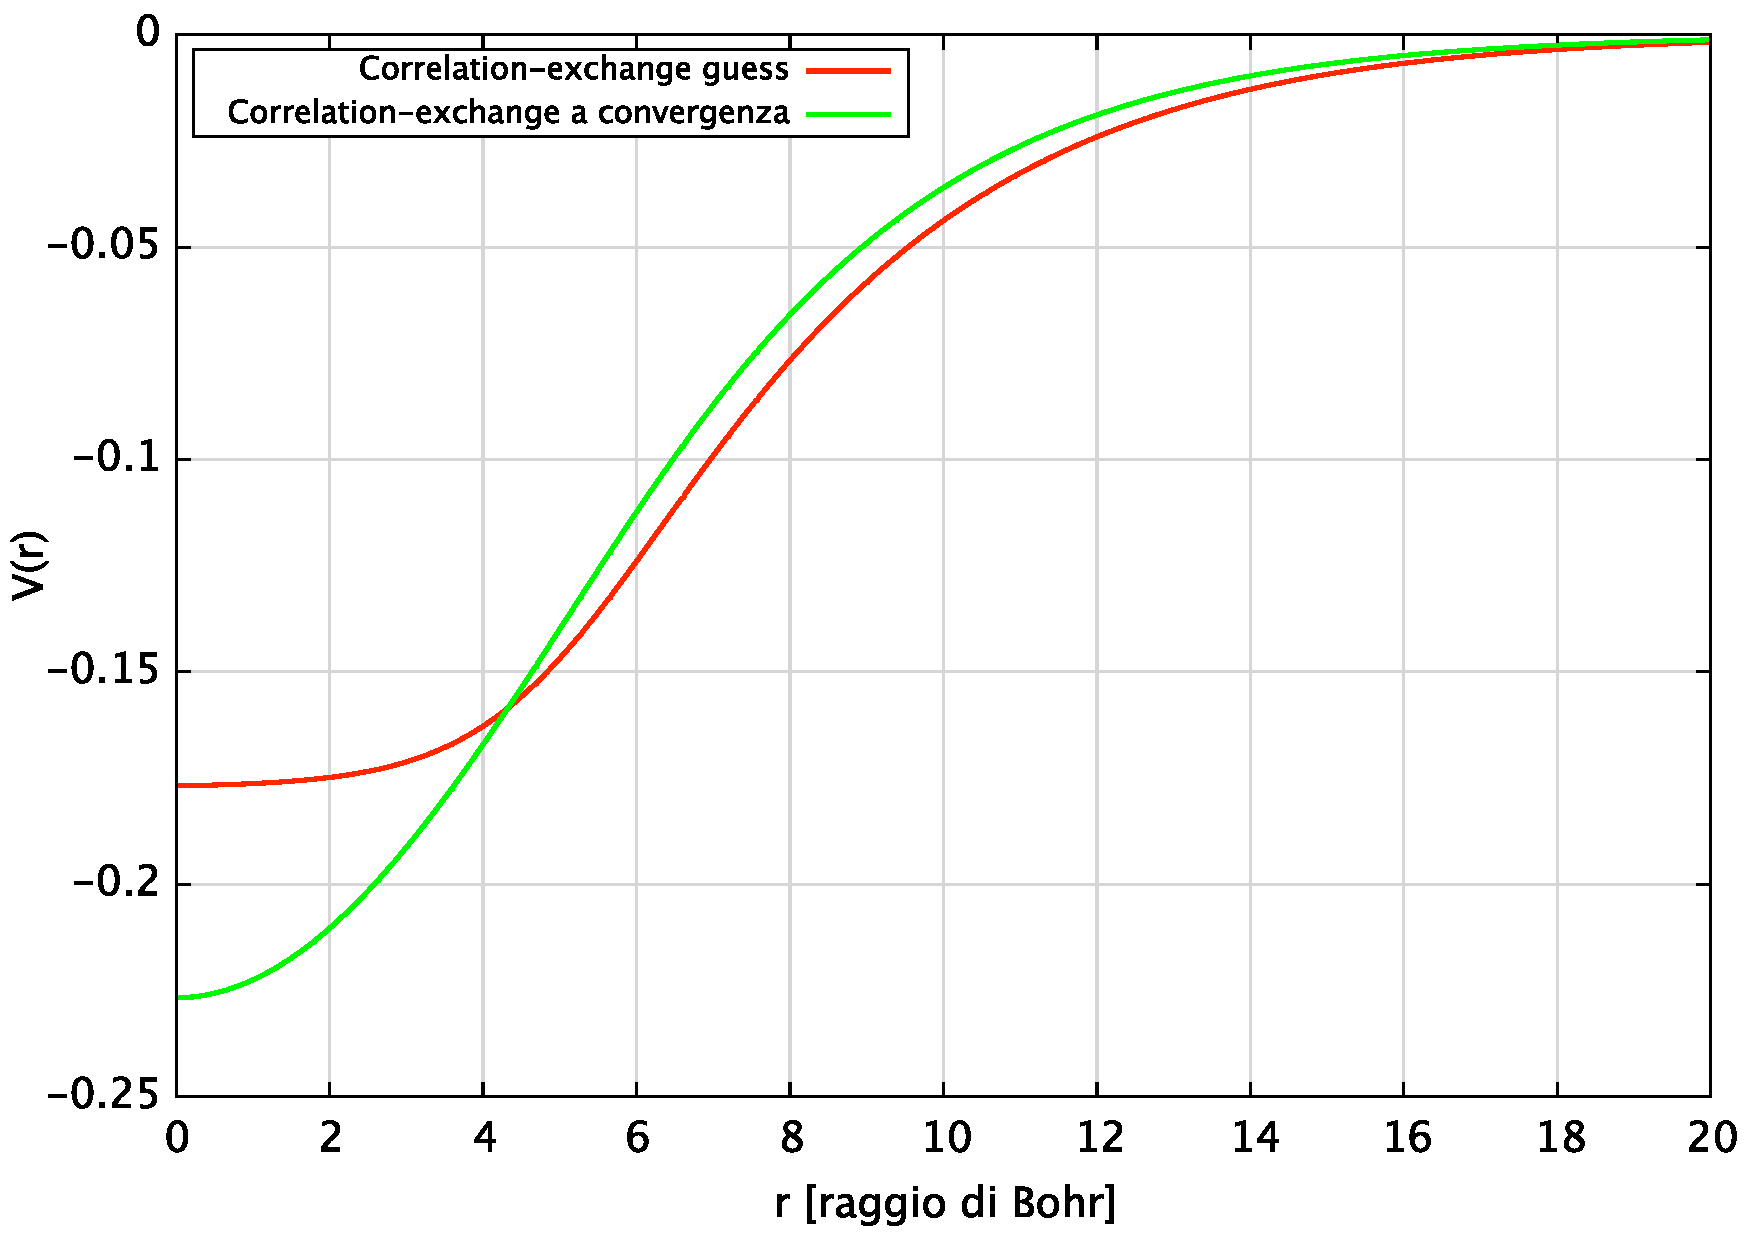
\includegraphics[scale=0.25]{Img/ce-2}}
\hspace{3mm}
\subfigure[$N=8$]
{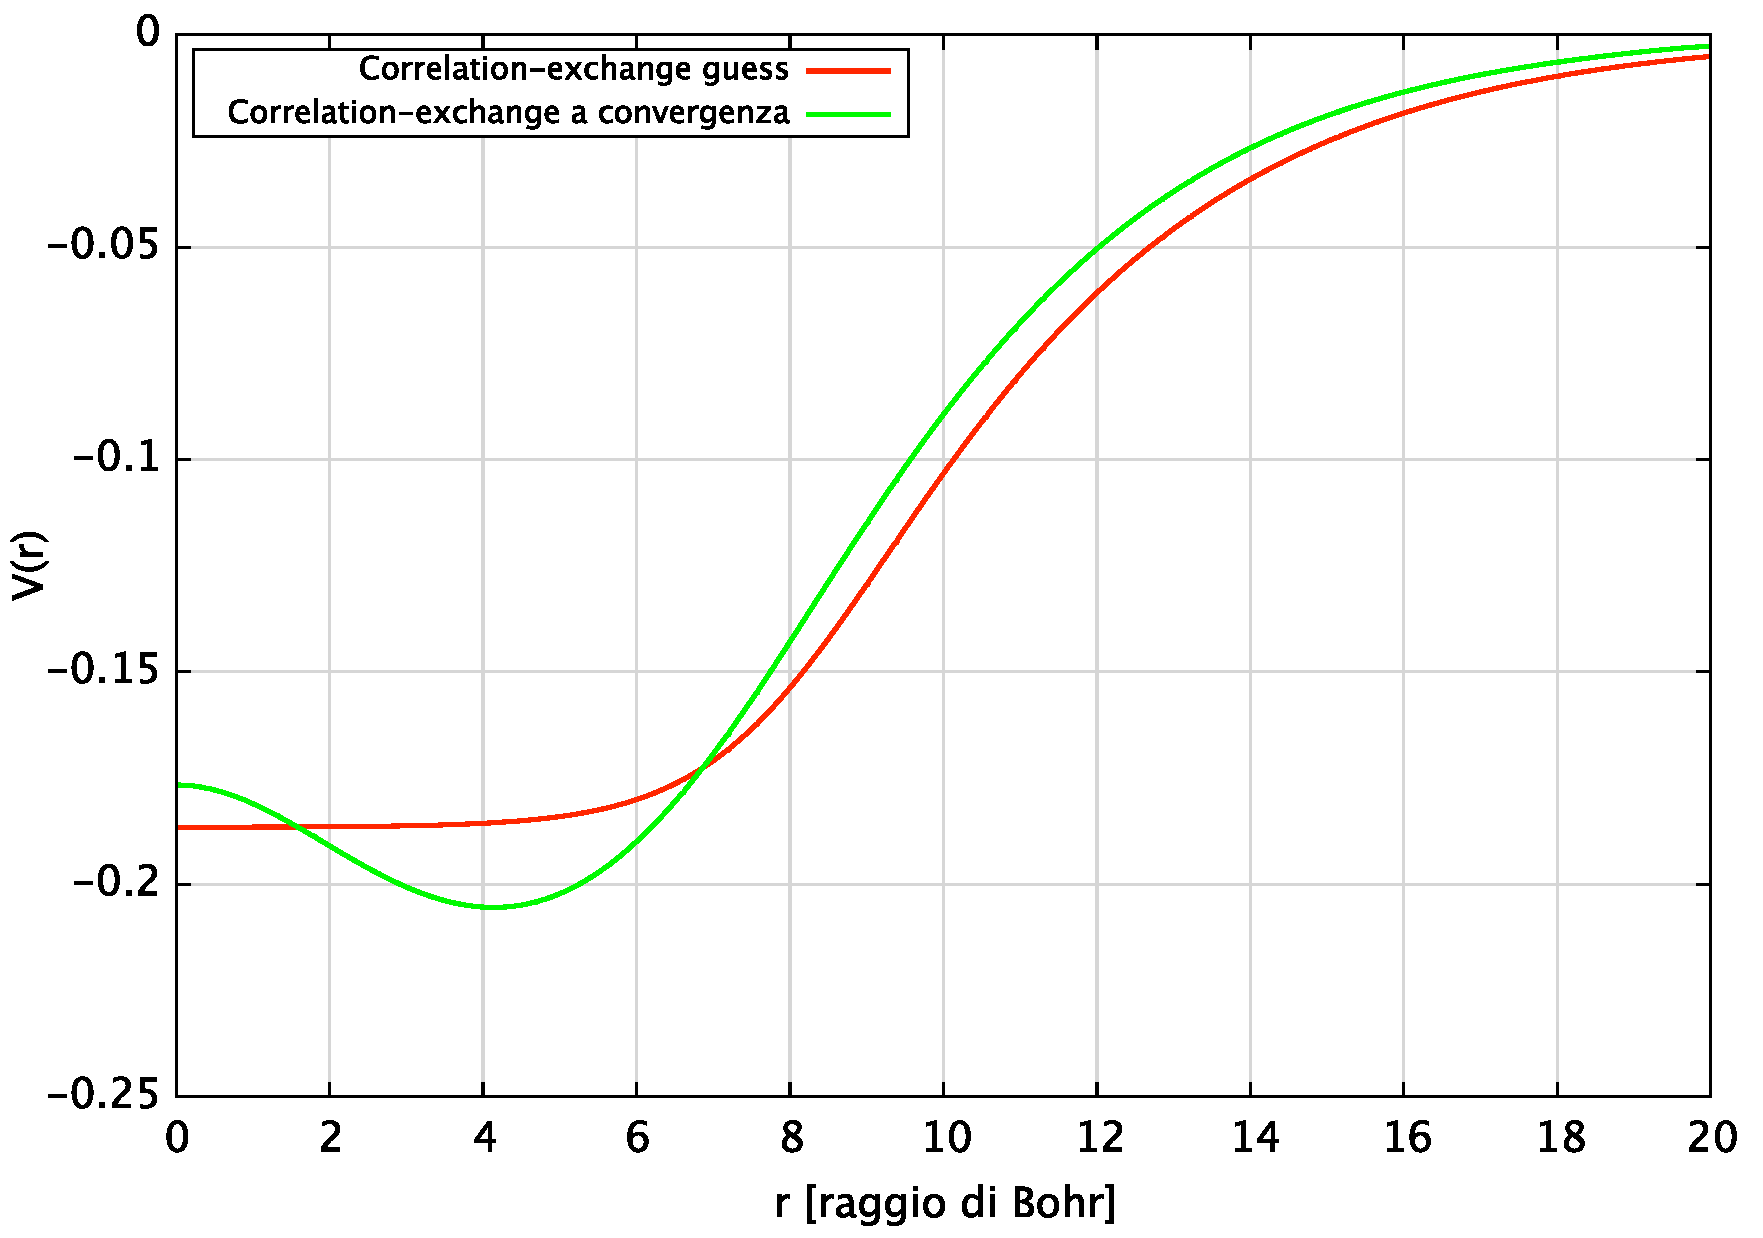
\includegraphics[scale=0.25]{Img/ce-8}}
\subfigure[$N=18$]
{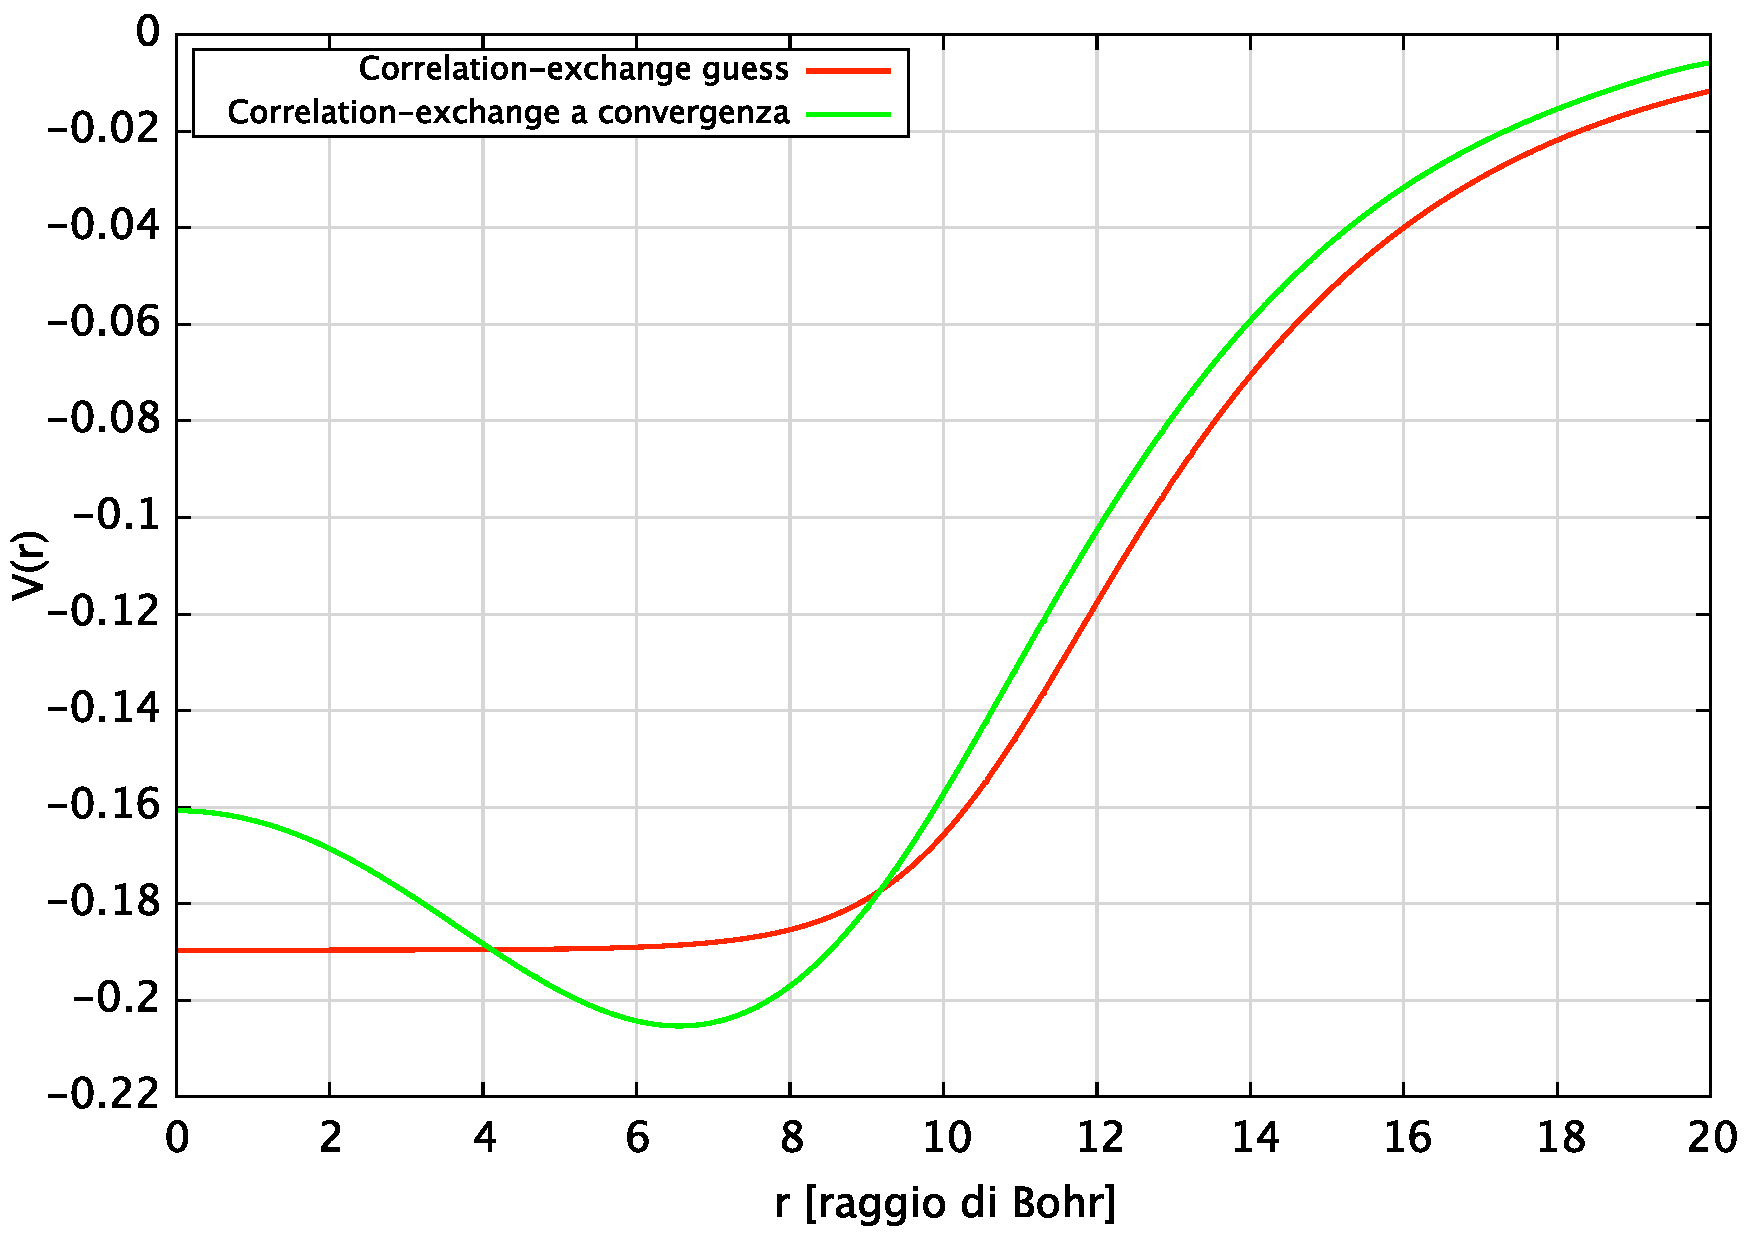
\includegraphics[scale=0.25]{Img/ce-18}}
\hspace{3mm}
\subfigure[$N=20$]
{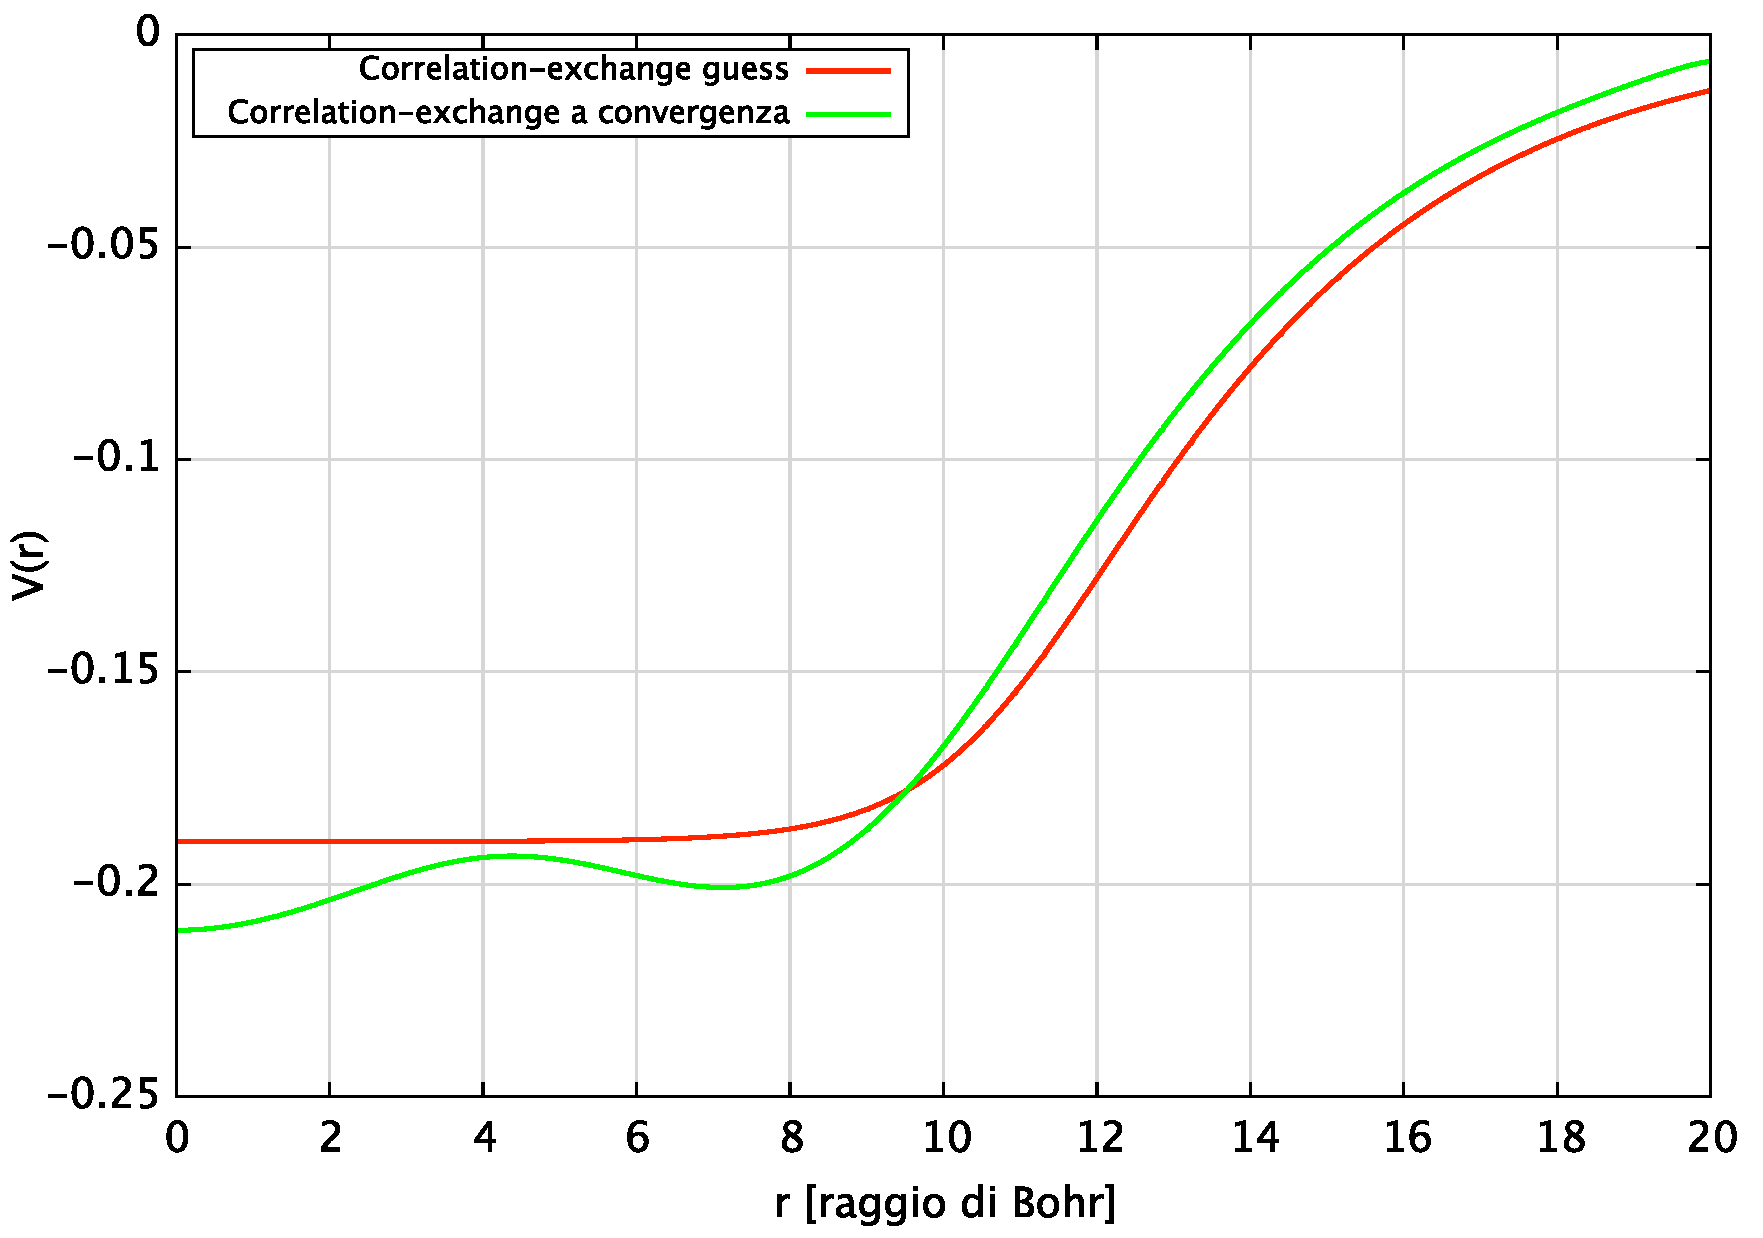
\includegraphics[scale=0.25]{Img/ce-20}}
\subfigure[$N=34$]
{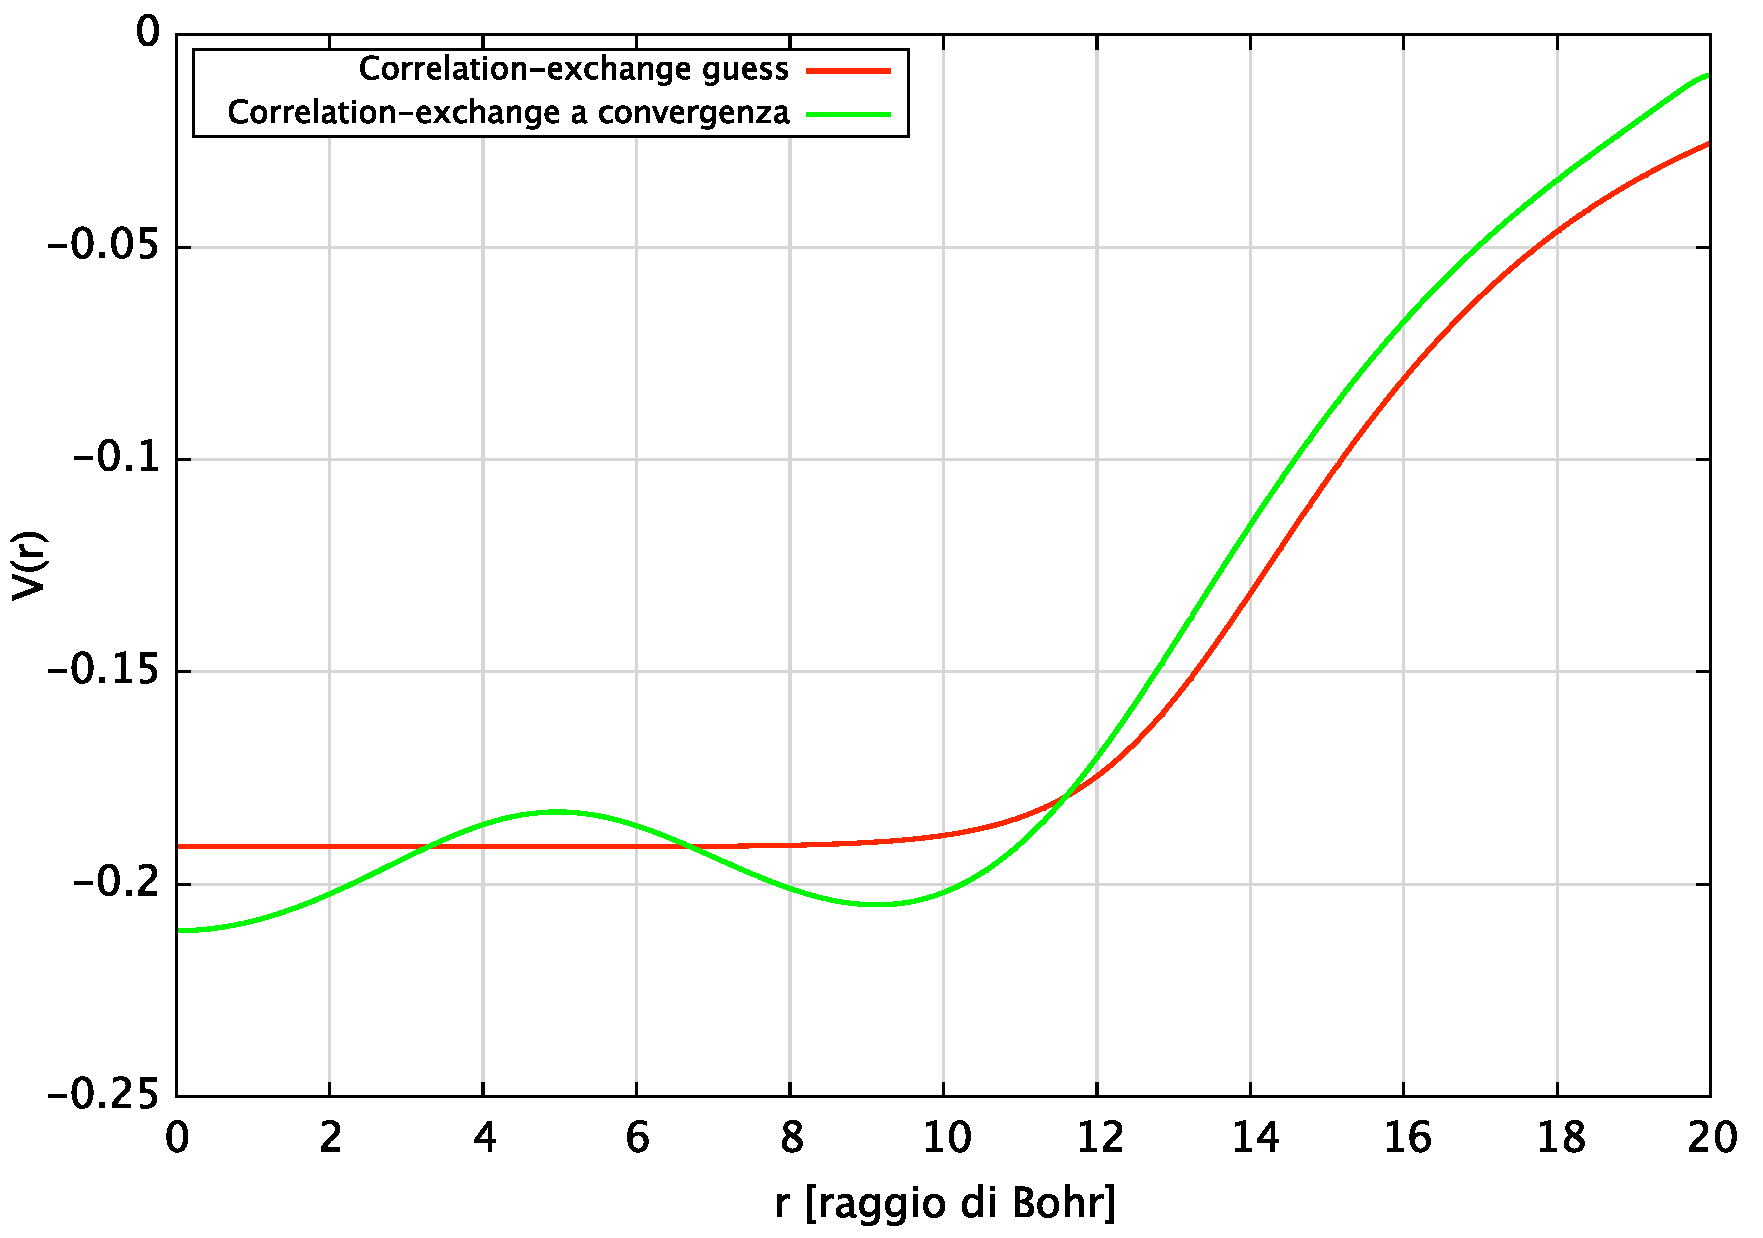
\includegraphics[scale=0.25]{Img/ce-34}}
\hspace{3mm}
\subfigure[$N=40$]
{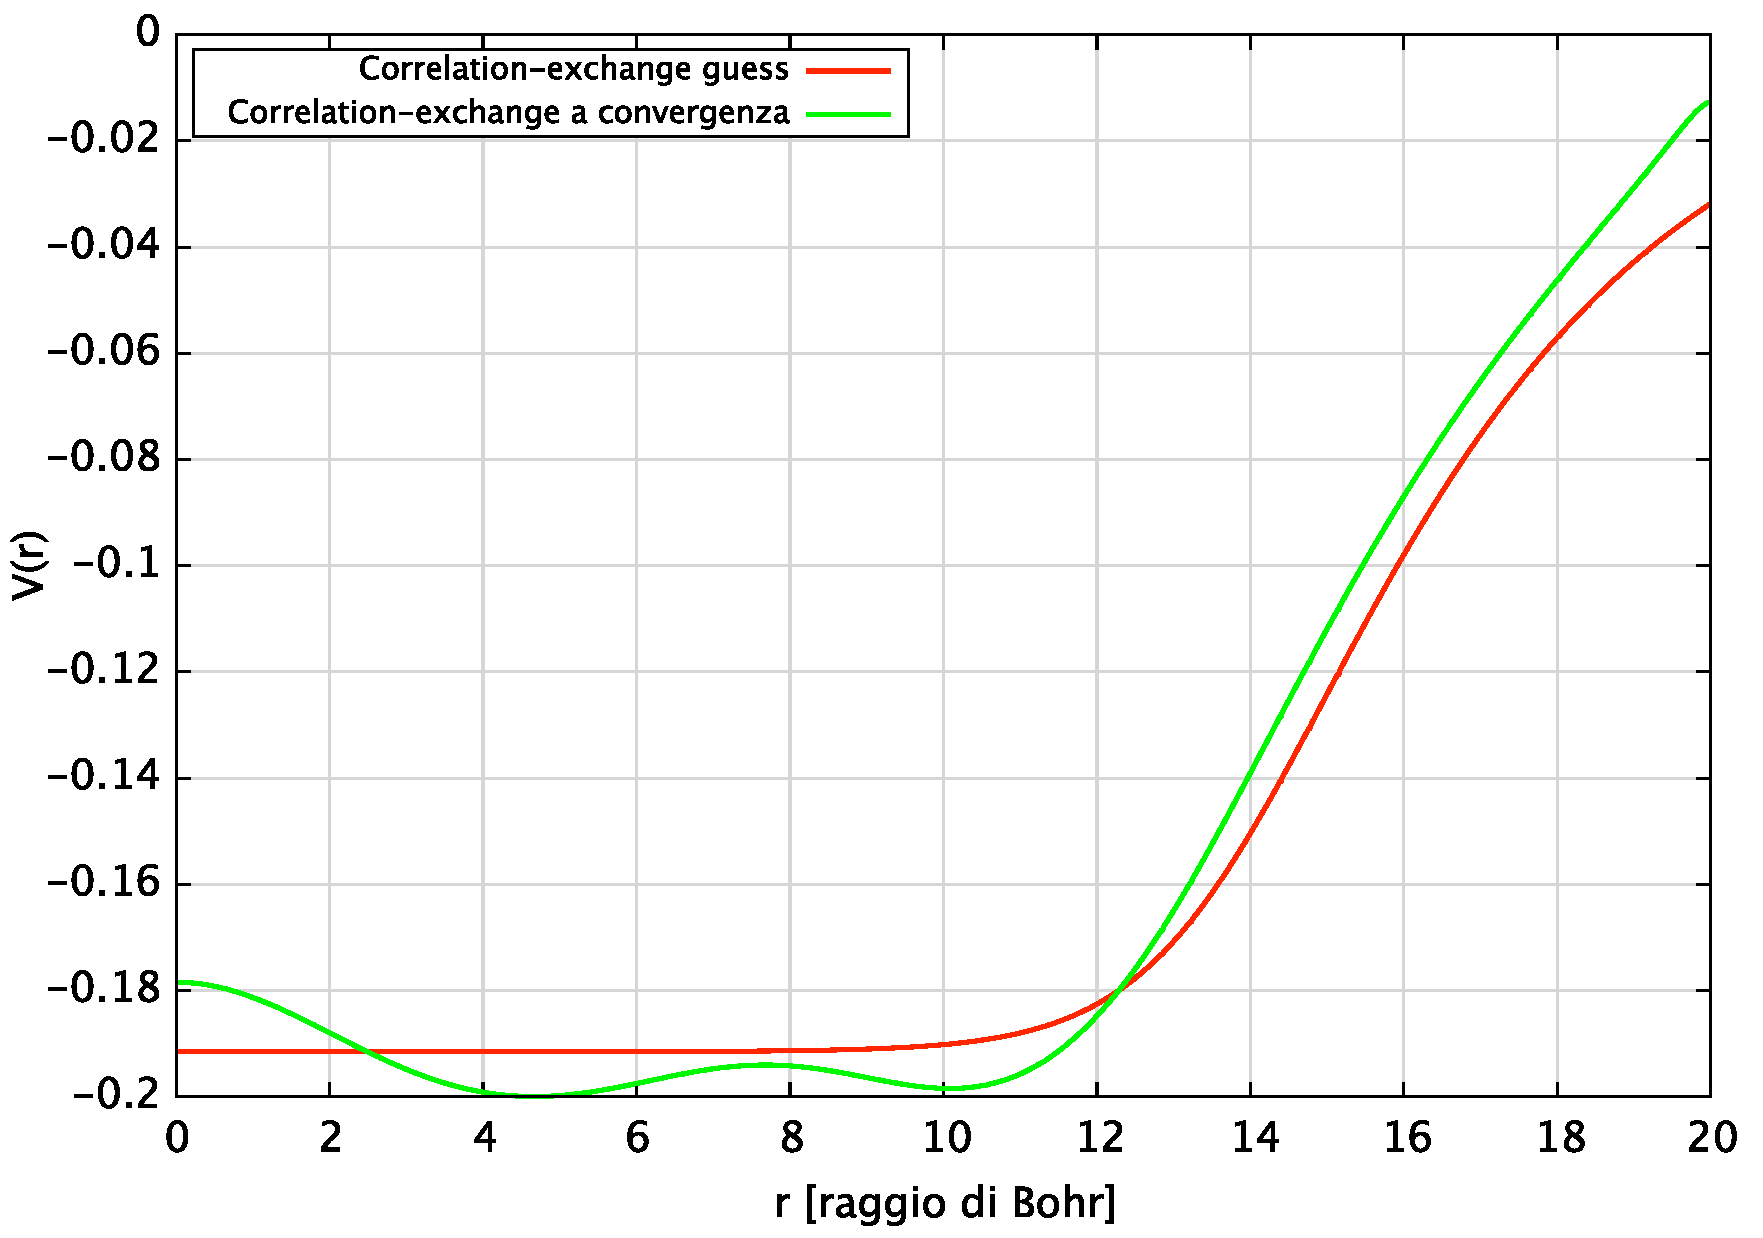
\includegraphics[scale=0.25]{Img/ce-40}}
\caption{Plot del potenziale di scambio-correlazione del sistema fermionico nelle diverse configurazioni a shell chiusa}
\end{figure}\ \\

Infine mostriamo un immagine dell'andamento delle energie di singola particella corrispondenti alle diverse configurazioni a shell chiusa (immagine che può essere confrontata con Fig. 2.3 (a) di [1]):
\newpage

\begin{center}
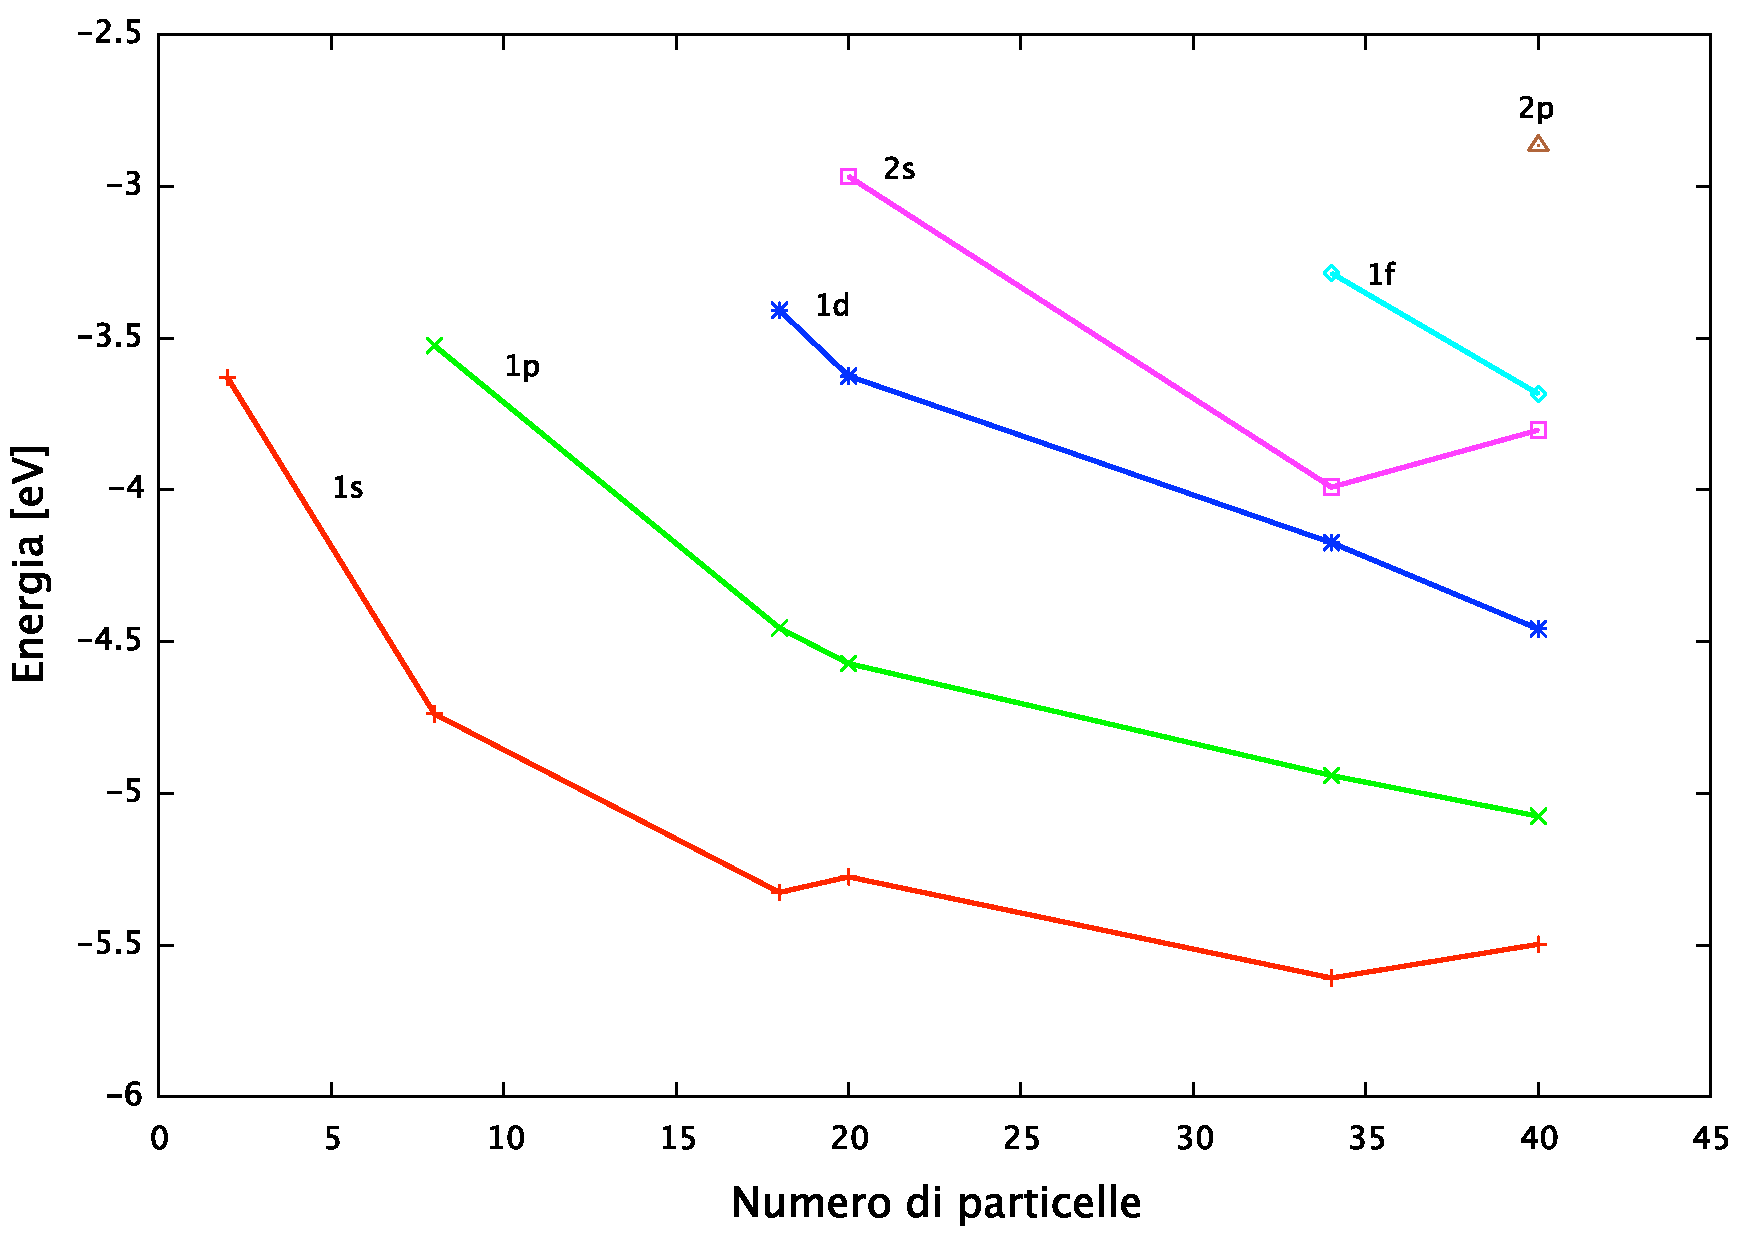
\includegraphics[scale=0.4]{Img/spe}
\end{center}
Possiamo osservare che le energie di singola particelle non mostrano un comportamento a shell particolarmente marcato in corrispondenza dei numeri magici: questo rimarca il fatto che le equazioni di Kohn-Sham (quantomeno in approssimazione di densità locale) non sono uno strumento adatto alla previsione di energie di singola particella, quanto piuttosto al calcolo dell'energia complessiva del sistema. 


\end{document}